% NOTES 
% Wie ich den sprinback gemssen habe 

\chapter{Build}\label{ch:build}
This chapter outlines the steps of the \ac{DSR} process, which are
summarized under the ``Build'' phase, as described chapter~\ref{ch:research-methodology}
resarch methodology.
The first step in this phase is to identify the problem that need to be addressed,
this step leads to the formulation of \ac{DP}, which are later used to evaluate
the effectiveness of the artefact.
The \ac{DP} are derived from the requirements of the overall models and are based on
the work of~\cite{siebert2022construction}.

The Build phase involves the creation of machine learning models, which serve as
artifacts.
By implementing these steps, the DSR process establishes a rigourous and methodical
approach for creating new artifacts.


\section{Problem Identification and Motivation}\label{sec:problem-identification-and-
motivation}

For several decades, researchers have been conducting extensive research on sheet metal
forming technologies in response to the growing demand for lightweight metal components.
One of the challenges is the phenomenon of spring back, as discuessed in~\ref{sec:spring-back}.
As a result, various efforts have been made to devise methods for compensation~\cite[p.1]{
    liu_newmachinelearning_2012}.

Sheet metal forming is a complex process due to non-linear behavior caused by
deformations of the metal sheet, making the spring back difficult to predict.
Consequently, conventional methods often employ trail and error approaches~
\cite[p. 1]{dib_singleensembleclassifiers_2020}.
Through speaking with experts of the field of sheet metal forming, it was found that
a usual trial and error approach is the creation of so called ``technology tables'' that
contain the bending parameters and resulting spring back data. An example of a table can be seen
in the appendix~\ref{sec:technology-table}.
These tables are produced by conducting numerous experiments with varying bending
angles and metal sheets.
However, this process is time-consuming and costly, making it
unsuitable for the production of high-volume and low-cost components (personal communication, Dr
. Wolfram Hochstrate and M. Sc. Peter Lange).

In conclusion, the findings suggest the necessity of a \ac{ML} model to predict spring
back accurately.


\section{Objectives of a Solution}\label{sec:objectives-of-a-solution}
The design principles used to evaluate the machine learning (ML) models in \ac{DSR}
process and form the objectives of the solutoin.
work are based on a selection of quality parameters proposed by
Siebert et al.~\cite{siebert2022construction}.
These quality parameters have been tailored specifically for the evaluation of ML
models and are thus well-suited to the evaluation of the models developed in this
thesis.

\subsubsection*{Design Principle 1: Correctness}
\textit{"Does the artifact predict the spring back of a sheet metal with a
high accuracy and
correctness?"}~\cite[p. 16]{siebert2022construction}

The demand for high-quality products is a driving force in the manufacturing industry,
as consumers and businesses alike demand products that meet stringent standard of
precision and accuracy.
This is particularly true in the case of sheet metal forming, where even small
deviations from the desired dimensions can cause significant implications for the final
product.
Therefore, metal parts need to be produced with high precision and accuracy and
spring back is an undesired side effect which needs to be minimized~\cite[p.1]{
    cruz_applicationmachinelearning_2021}.

\ac{ML} has emerged as a powerful tool for predicting the spring back in other bending
methods as shown in section~\ref{sec:state-of-research}~state of research.
A \ac{ML} model should predict the spring back with a high degree of accuracy and
correctness, as even small errors in the prediction will cause fitting problem in the
manufacturing process.

\subsubsection*{Design Principle 2: Relevance}
In addition to measure the correctness it is important to understand ``why''
the learner has this performance.
A model is considered relevant when it is able to accurately predict the outcomes of
new unseen data, that were not used during training.
A relevant model should have a low error rate on both the training data and the test
data and achieve a good bias-variance trade-off~\cite[p. 16]{siebert2022construction}.

Understanding the bias-variance trade-off is crucial in developing \ac{ML} models that
generalize well to unseen data~\cite[p. 49--51]{zhou_machinelearning_2021}.
In machine learning (\ac{ML}), achieving a good bias-variance balance is essential.
This means that a model can accurately capture the underlying patterns in the data
without overfitting or underfitting~\cite[p. 49--51]{zhou_machinelearning_2021}.

\subsubsection*{Design Principle 3: Robustness}

When working with real-world data, quality issues such as outliers, missing data, and
noise are common problems. These issues can have a negative impact on the performance
of the model, making it challenging to produce accurate predictions. To overcome these
challenges, a robust model must be able to handle data quality issues and still produce
accurate predictions~\cite[p. 16]{siebert2022construction}.

\cite{saez_evaluatingclassifierbehavior_2016} proposed a new measure called Equalized
Loss of Accuracy to evaluate classifications models for robustness.
Because regressions algorithms are used in this new metrics have to be found~\cite[p.
3]{saez_evaluatingclassifierbehavior_2016}.

\subsubsection*{Design Principle 4: Stability}

The stability of a model is an important quality parameter, as it is essential that
the model produces the same results when trained on different datasets.
This is particularly important in the case of \ac{ML} models, as the training data
is often limited and the model is trained on a small subset of the available data.
Therefore, it is important that the model is able to generalize well to unseen data and
produce repeatable results when trained on different datasets~\cite[p. 16]{
    siebert2022construction}.

\subsubsection*{Design Principle 5: Interpretability}

Interpretability refers to the ease with which humans can understand and make
sense of the decisions made by a trained machine learning model~\cite[p. 13]{
    molnar2020interpretable}.
\cite{miller2019explanation} define interpretability as the ``degree to which
a human can understand the cause of a decisio''~\cite[p. 1]{miller2019explanation}.
Good interpretability is important because it allows users to trust and rely
on the model, and it can also help with debugging and improving the model (\textit{
    Source}).

Interpretable models will also deliver more insights for this project, as the
goal is to understand the relationship between the features and the target outcome.

As mentioned in chapter~\ref{ch:theoretical-foundations} there are many parameters
and variables involved in the sheet metal forming process.
That makes the process design quite complex, particularly in the production
of components which require several stages, and thus more than one set of tools~\cite[p.
1]{dib_singleensembleclassifiers_2020}.
A interpretable model which allows conclusions how the results where generated is better.

\subsection*{Design Principle 6: Resource utilization}
One of the primary objectives of utilizing machine learning for predicting spring back is to
reduce the number of trial-and-error cycles during the manufacturing process, thus saving
valuable resources such as material and labor (refer to Section~\ref{sec:problem-identification-
and-motivation}).
Typically, a technology table requires 11 or more bends in a single sheet of metal, all with the
same thickness.
Unfortunately, these metal sheets cannot be repurposed due to their specific angles,
resulting in wasted materials and manual labor.
Moreover, the machines used for bending the metal
are often occupied around the clock, further adding to the inefficiency of the process (
personal communication, Dr. Wolfram Hochstrate).

Nevertheless, it is crucial to acknowledge that developing an ML model also entails resource
consumption.
Training \ac{ML} models can be a labor-intensive process, as it often requires significant
computing power and the generation of large amounts of training data, depending on the algorithm
used.
Furthermore, making predictions using an \ac{ML} model also requires computing power.
Therefore, it is crucial to carefully consider the resources needed to train and use the model
effectively~\cite[p. 16]{siebert2022construction}.
What resources are used and evaluated is described in more detail in~\ref{sec:resource-
utilization}.


\section{Dataset generation}\label{sec:dataset-generation}

To generate the dataset, bending experiments on metal sheets of varying
thicknesses where conducted.
Specifically, cold rolled steel sheets that conform to the DIN EN
10130 with thicknesses raning from 0.5 mm to 3 mm where used.
The material was selected because it is commonly used in bending processes and widely
available.
To create the dataset, pieces of the material were cut into 20×100 mm pieced each piece
was bent using a Zwick three-point-bending machine.
It was paid attention to ensure that each metal sheet was bent in the same
rolling direction as preliminary tests showed that the spring back differed depending
on the rolling direction.

The dataset consisted of 384 \texttt{.tra} files which is a proprietary format used by
the machine.
Python script where developed to covert the output data format from the
machine to CSV files.

The following describes the experimental setup used for the experiments
performed.
The data collection was done outside of the thesis period and originally consited of 384
samples. \texttt{X} samples where added later to the dataset to fill gaps present in
the dataset.

% Pado: Since the data collection was technically done outside of the thesis
% period, 4.2.1
% (Multiple cycles) can be
% omitted. 4.2.2 is needed in order to understand the data set.

%\subsection{Preliminary Tests}
%A number of preliminary tests were conducted to determine the influence of
%the punch penetration
%on the spring back.
%
%\subsubsection{Multiple Cycles}
%One approach was to test if multiple spring back can be measure using only
%one sheet.
%Therefore, the machine was programmed to perform multiple cycles in one
%attempt and bend the
%metal sheet multiple
%times. The benefit of this approach would have been a faster generation of
%the dataset because
%spring backs could be
%measured in on attempt, also less material would have been used.
%
%Figure~\ref{springback_multiple} shows one of these attempts. The metal
%sheet was bent 4 times
%using $y_p$ values
%from 5 to 8. The results show, that 4 different spring backs can be
%measured, but the spring back
%does not vary like
%expected. It was observed as well, that the spring backs are different in
%every attempt, this is
%shown in
%Figure~\ref{springback_multiple_inconsistent_results}.
%Bending 4 different metal sheets each only one time returned very different
%results.
%A possible explanation could be the cold deformation of the steel, which is
%not reversible.
%Because this approach did
%not work, the machine was programmed to perform one cycle at a time.
%
%\captionsetup{width=0.45\textwidth}
%
%\begin{figure}[H]
%    \centering
%    \begin{minipage}[b]{0.5\textwidth}
%        \centering
%        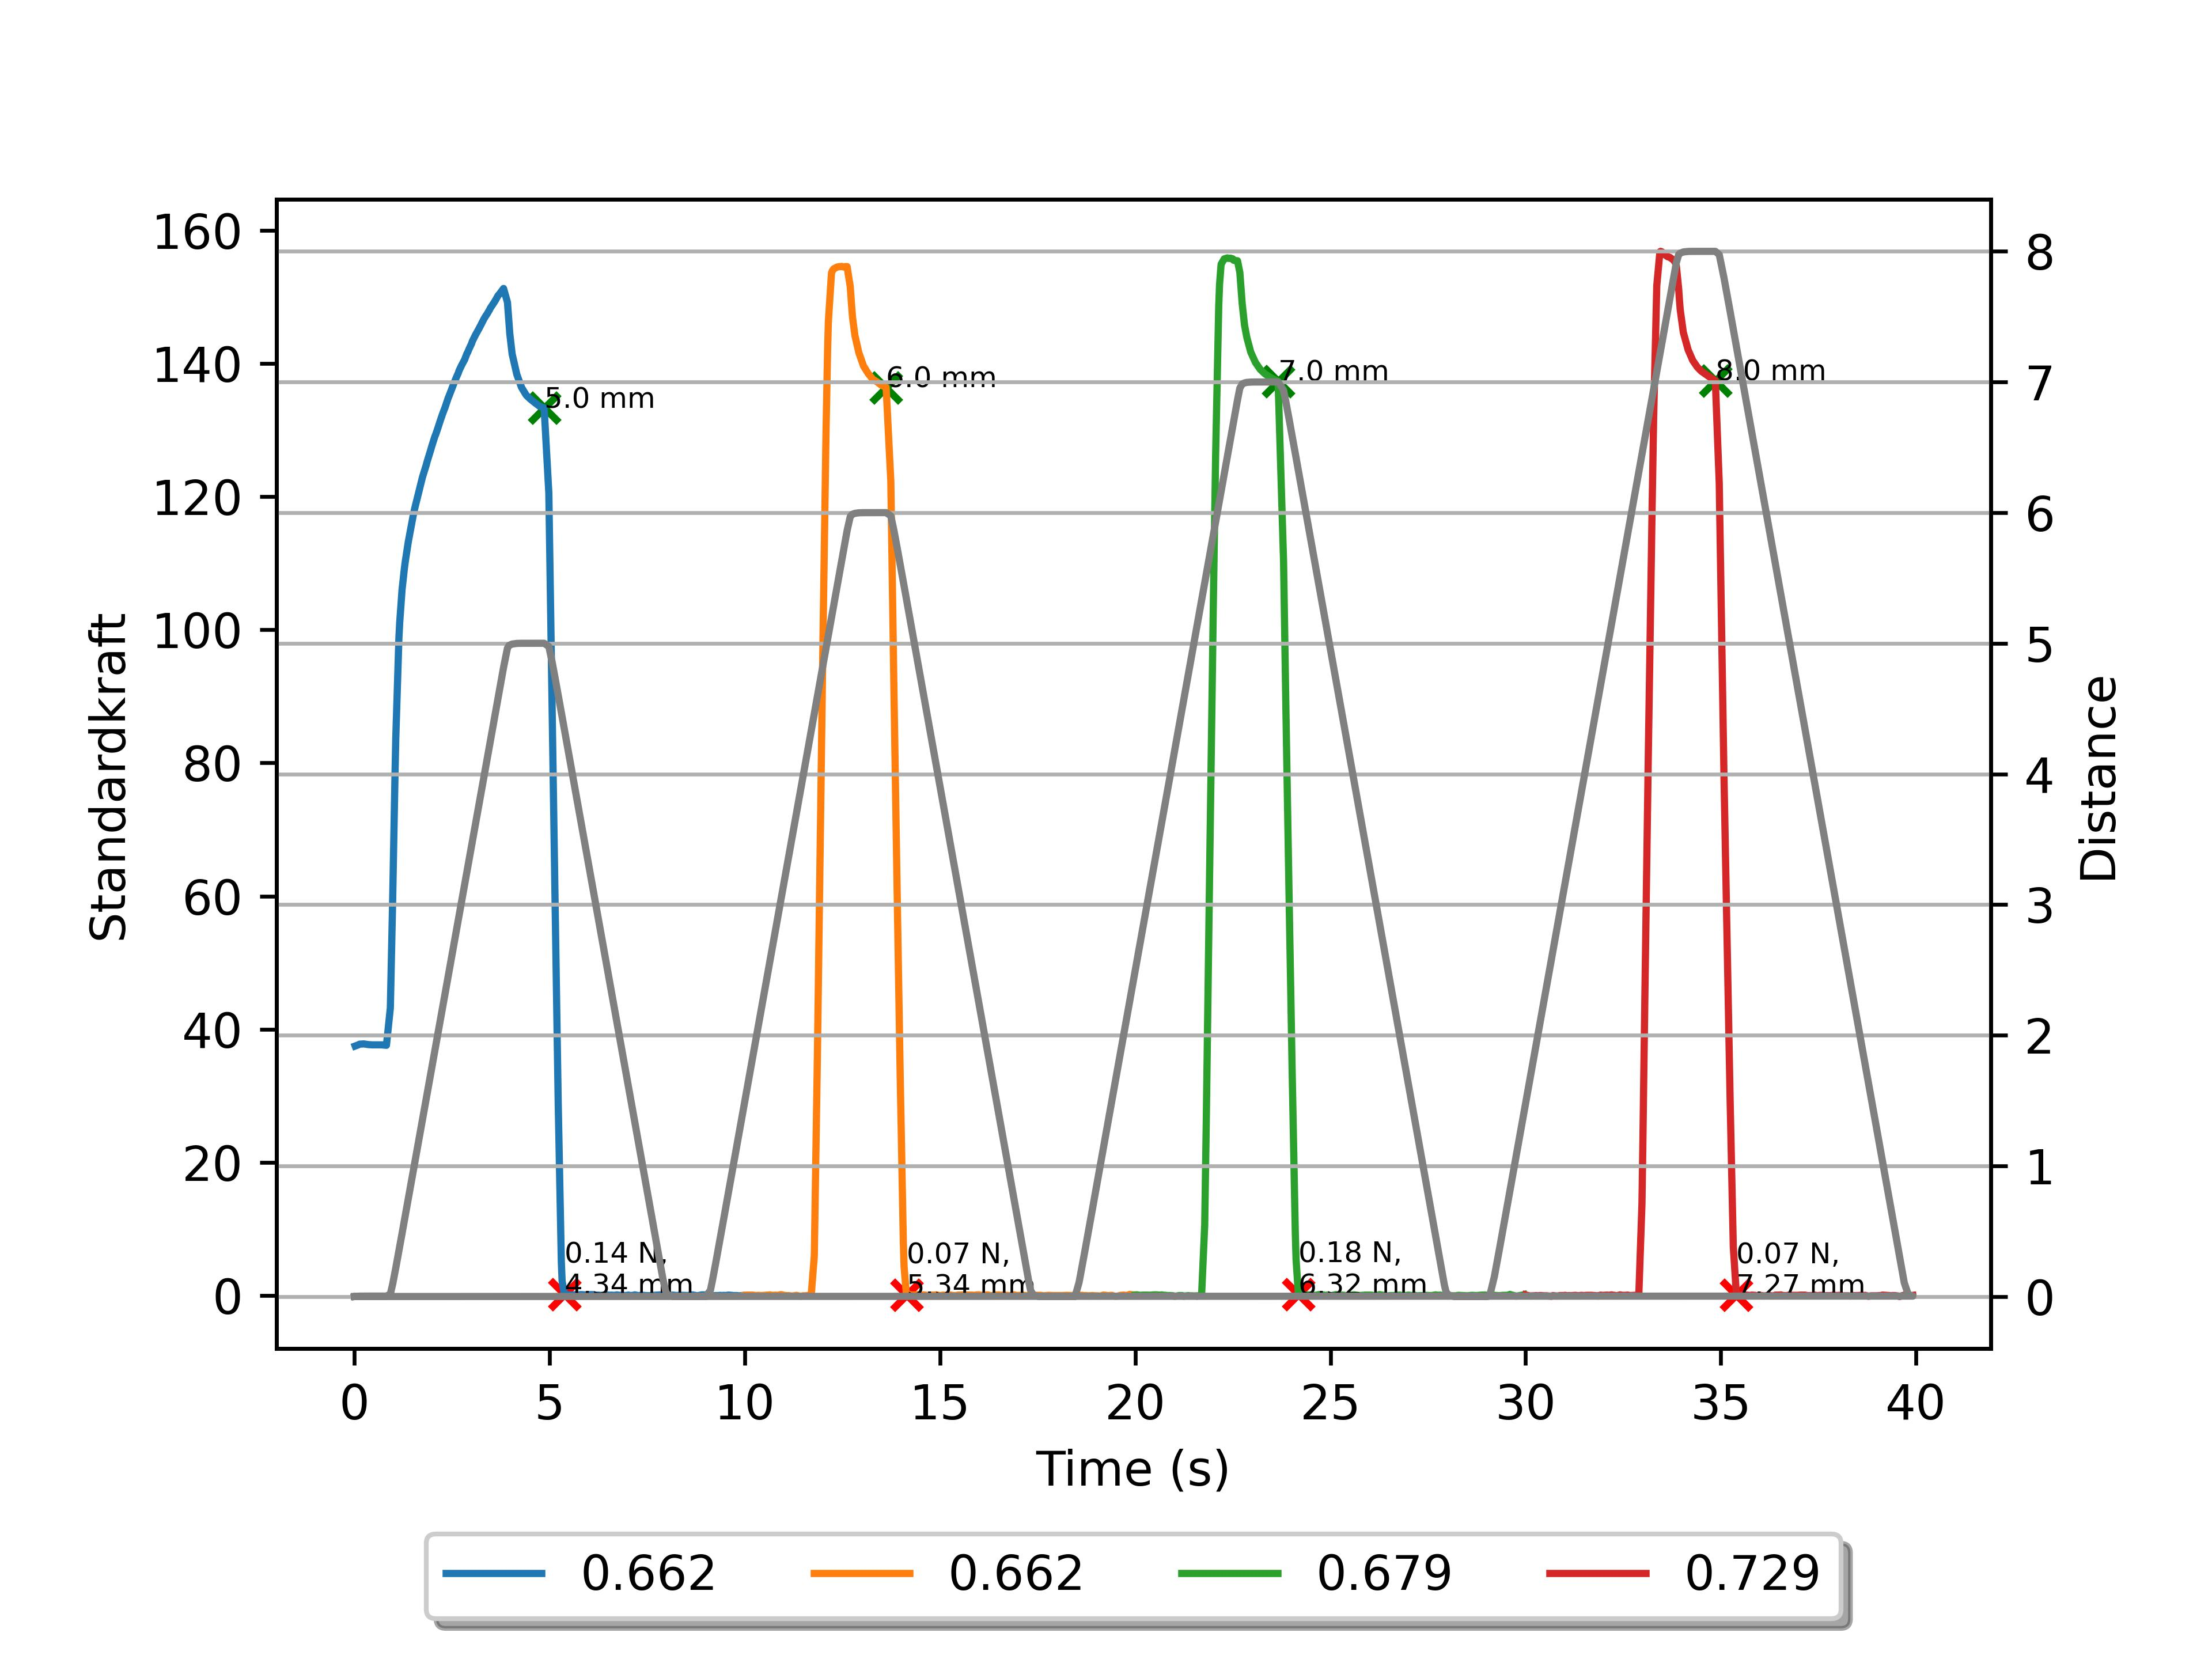
\includegraphics[width=0.9\textwidth]{springback_multiple.jpg} %
%first figure itself
%        \caption{Experiment: Bending one metal sheet multiple times with
%different $y_p$ values.}
%        \label{springback_multiple}
%    \end{minipage}\hfill
%    \begin{minipage}[b]{0.5\textwidth}
%        \centering
%        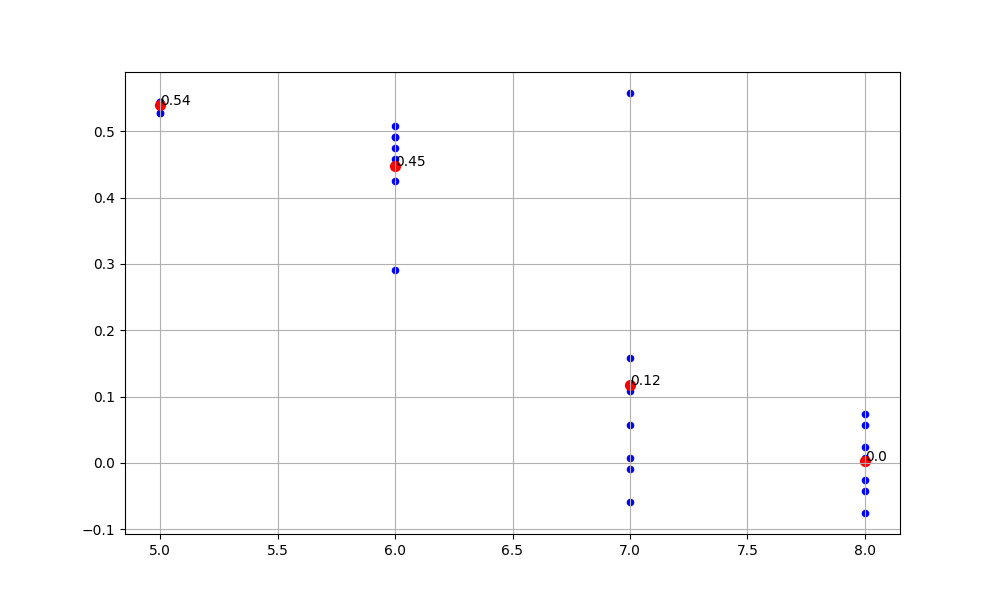
\includegraphics[width=1
%.1\textwidth]{springback_multiple_inconsistent_results.png} %
%        second figure itself
%        \caption{Inconsisten results bending one metal sheet mutliple times.
%The spread of the
%        results is very large.}
%        \label{springback_multiple_inconsistent_results}
%    \end{minipage}
%    \label{fig:springback_multiple_overview}
%\end{figure}

%\subsubsection{Bending Machine}
%Before using the three point bending machine, a brake bending machine was
%used to test the
%influence of the bending
%on the spring back. The brake bending machine is a machine used to bend
%metal sheets. It is a
%very common machine in
%the industry and is used to bend metal sheets to a specific radius. The
%brake bending machine
%used is a
%\textit{Bendmaster 1000} from \textit{Bendmaster}.
%
%After a series of bends it was observed, that the spring back values where
%much higher than
%expected. The explanation
%for that behavior was, that altering the position the bending beam of that
%specific machine was
%not enough to get the
%desired angle. Thus, the machine excluded for the generation of the data and
%the three point
%bending machine was used
%instead.
%
%Despite the inaccurate data, it was later observed, that the distribution of
%the spring backs was
%very similar to the
%later experiments with the three point bending machine.

\subsection{Experimental setup}\label{subsec:experimental-setup}
The experimental setup comprises of a three-point bending machine, consisting
of a punch and die, with the latter lacking a bottom, which allows only air bending.

The material testing machine utilized is the \textit{Zwick 1454MO}, which is
equipped with a load cell and a displacement sensor.
The load cell measures the force applied to the sheet measured in $N$), while the
displacement sensor measures the displacement of the punch, denoted as $y_p$.
The punch is mounted on the top of the machine and is stationary, while the
die is mounted on the bottom and is the part which can be moved.
The die opening of the machine is adjustable with from 10mm to 100 mm.
The machine is operated via a computer and the \textit{ZwickRöll TestXpert} software,
which is used for both machine control and data collection.

The experimental setup and the process parameters are shown in
Figure~\ref{fig:process_parameters} where $V$ is the die opening which is the
opening of the two contact points on which the sheet metal is placed.
The parameter $y_p$ is the punch penetration, which is the distance the punch is moved
into the sheet.
The metal sheet thickness is donated as $t$ and the bending angle as $\alpha$.
The parameter $r_p$ is the radius which of the tip of the punch, which was never
replaced in the experimental setup and therefore remains constant.

\begin{figure}[h]
    \begin{tcolorbox}[arc=0pt,boxrule=0.5pt]
        \centering
        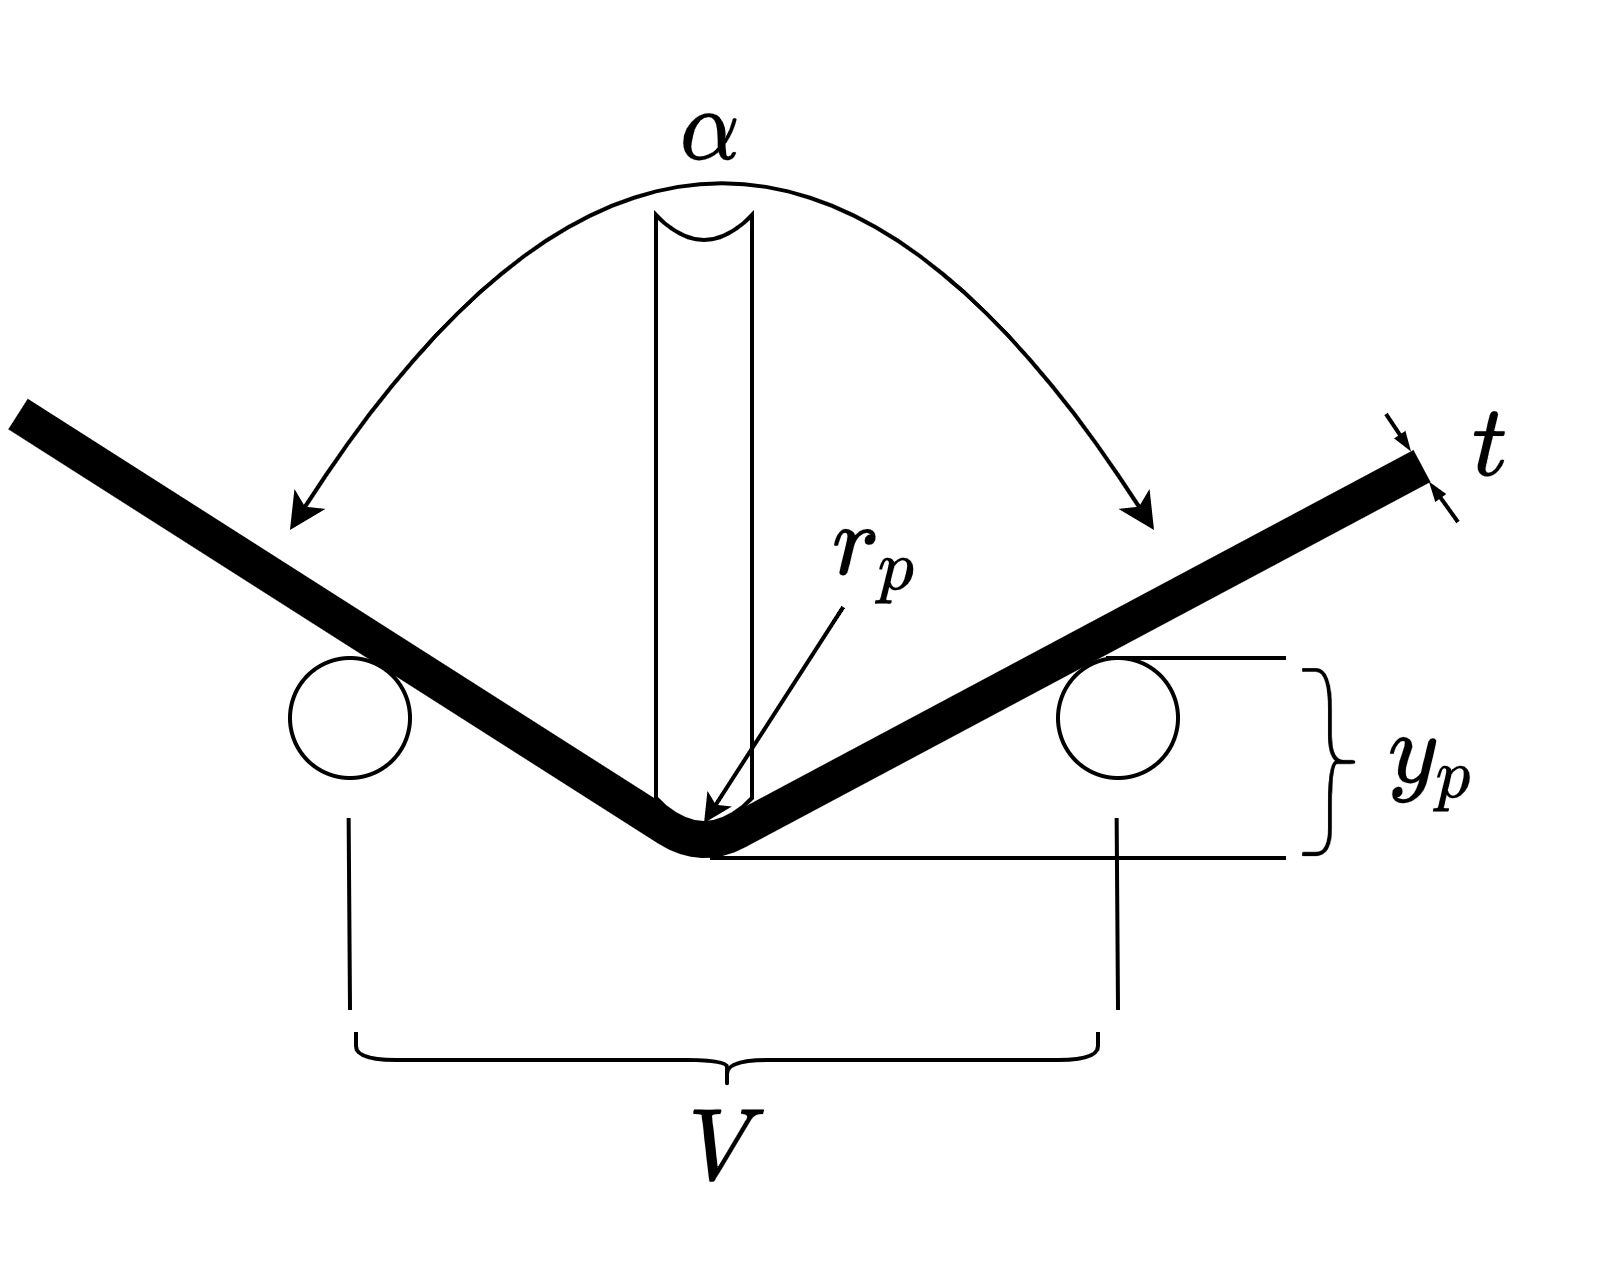
\includegraphics[trim=left botm right top, width=0.6\textwidth,
            clip]{process_parameters}
        \caption{\textbf{Process parameters:} Sheet bending angle ($\alpha$), sheet
        thickness ($t$), punch
        penetration ($y_p$), die opening ($V$) and punch radius ($r_p$)}
        \label{fig:process_parameters}
    \end{tcolorbox}
\end{figure}


To ensure consistent results, a set of constant and variable parameters were selected.
The constant parameters consisted of the punch-and-die tooling made of steel, which
included the die punch radius (r_p), as well as the length and width of the
metal sheet. Additionally, the punch travel speed, hold time, and punch force threshold
were also considered constant.

All metal sheets used in the setup were standardized with a length of 80 mm and a width
of 20 mm.
The hold time, which refers to the duration that the punch remains stationary
after reaching the maximum displacement ($y_p_{\max}$), was set to a minimum of 1 second.
The punch force threshold was set to 1 N, meaning that the punch was initially moved at
a higher speed until the force reached 1 N, and then moved at a slower speed of 80 mm
/min until the $y_p_{\max}$ was reached.


\begin{table}[htb]
    \begin{tcolorbox}[arc=0pt,boxrule=0.5pt]
        \sisetup{group-minimum-digits = 4}
        \centering
        \label{tab:experimental-setup-constant-parameters}
        \begin{tabular}{lll}
            \toprule
            \thead{\textbf{Parameter}} & \thead{\textbf{Values}} &
            \thead{\textbf{Unit}}
            \\
            \midrule
            Punch radius & 5 & $mm$
            \\
            \hdashline
            Sheet width & 20 & $mm$
            \\
            \hdashline
            Sheet length & 100 & $mm$
            \\
            \hdashline
            Punch speed & 80 &
            $mm/min$ \\
            \hdashline
            Punch speed up (after bend) & 8 &
            $mm/min$ \\
            \hdashline
            Hold time & 1 & $s$ \\
            \hdashline
            Punch force threshold & 1 & $N$
            \\
            \bottomrule
        \end{tabular}
        \caption{Constant parameters in th eperimental setup}
    \end{tcolorbox}
\end{table}

The experiment involved varying three parameters: the die opening ($V$), the maximum
punch penetration ($y_p$), and the thickness of the metal sheet ($t$). The die opening
was varied from 10 mm to 50 mm, while the maximum punch penetration was varied from 2
.5 mm to 20 mm. The thickness of the metal sheet was also varied, with values ranging
from 0.5 mm to 2 mm.
These parameters and their values can be seen in Table~\ref{tab:experimental-setup-
variable-parameters}.

\begin{table}[htb]
    \begin{tcolorbox}[arc=0pt,boxrule=0.5pt]
        \sisetup{group-minimum-digits = 4}
        \centering
        \label{tab:experimental-setup-variable-parameters}
        \begin{tabular}{lll}
            \toprule
            \thead{\textbf{Parameter}} & \thead{\textbf{Values}} &
            \thead{\textbf{Unit}}
            \\
            \midrule
            %  \unit{(Kcal\per\mole)\squared}}} & \thead{RMSD l.b.} &
            %  \thead{RMSD u.b.}  \\
            \midrule
            Punch penetration  $y_p$ & 2.5, 5, 7.5, 10, 12.5, 15, 17.5, 20 &
            mm \\
            \hdashline
            Die opening        $V$ & 10, 20, 30, 40, 50
            & mm \\
            \hdashline
            Thickness          $t$ & 0,5, 1, 1.5, 2, 2.5, 3
            & mm \\
            \bottomrule
        \end{tabular}
        \caption{Varying parameters in the experimental setup}
    \end{tcolorbox}
\end{table}

\subsection{Measuring The Spring Back} \label{subsec:measuring_the_spring_back}
The output data included various data points that were used to calculate the spring back.
Key parameters for this calculation were the force (``Standardkraft''), punch penetration
(``Standardweg''), and time (``Testzeit'').
Figure~\ref{fig:springback_measured}
illustrates these three parameters, with the blue line representing the force and the
gray line representing the punch travel.


In Figure~\ref{fig:springback_measured} it can be seen that the force jumps to around 10 N
as soon as the punch touches the metal.
This is the case because the travel speed of the punch is 80 mm/min which relatively fast.
It was set to that speed in order to reduce the time of the experiments.

The wait time at of 1 second $y_p_{max}$ is a limitation of the machine and can not be
changed and therefore is always a part of the experimental setup.
At $y_p_{max}$ force decrease bee seen in figure~\ref{fig:springback_measured}, which is most
likely due to released friction (personal communications with ...).

\begin{figure}[H]
    \begin{tcolorbox}[arc=0pt,boxrule=0.5pt]
        \centering
        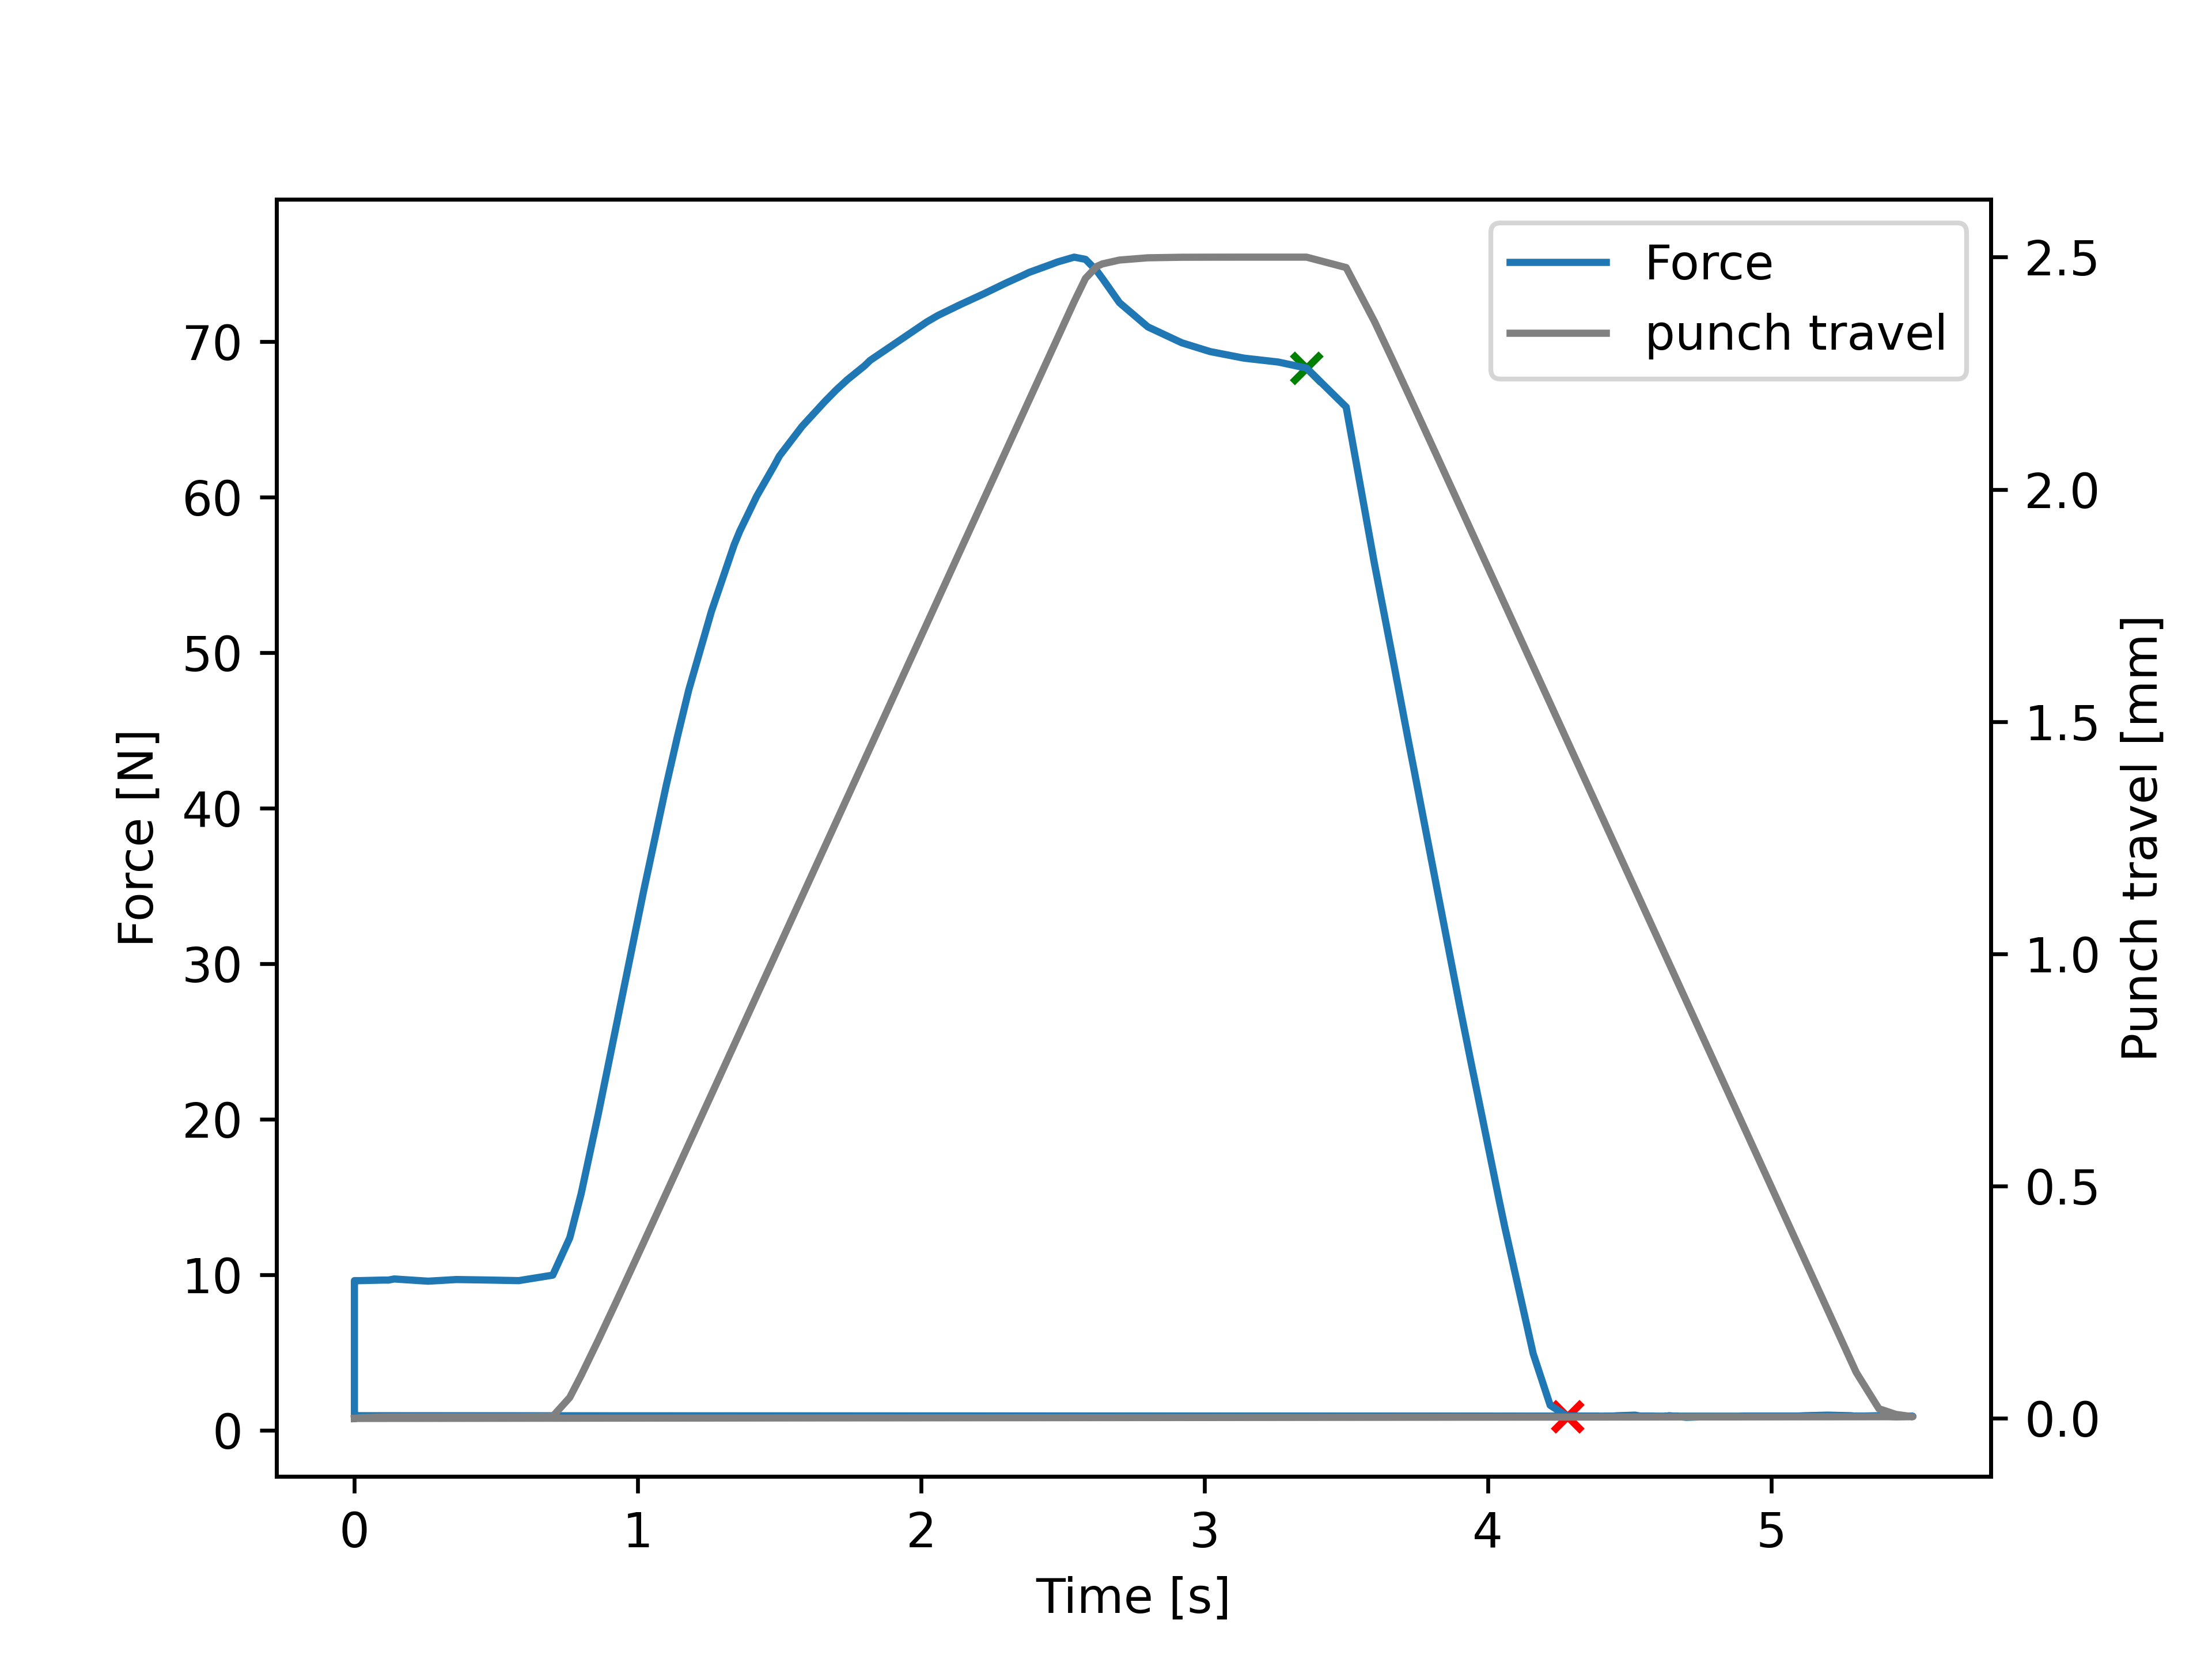
\includegraphics[width=0.9\textwidth]{springback_measured}
    \end{tcolorbox}
    \caption{A steel metal sheet was bent with a punch penetration of 5
    mm the spring back is 0 .37 mm. The blue line
    shows the force and the blue line shows the punch penetration.
    The distance between the green and the red point repesents the spring back distance.}
    \label{fig:springback_measured}
\end{figure}

\subsection{Dataset Exploration}\label{subsec:dataset-exploration}
The dataset was explored using the python library \textit{pandas}
\cite{mckinney-proc-scipy-2010} and the \textit{matplotlib}~\cite{Hunter:2007} library.
The goal of this section is to give the reader an overview of the dataset and
to show the relationship between the features and the dependent variable.

\subsubsection{Features}
The output data of the bending machine consisted of 26 features, which are listed in
the appendix.
Only three features - force, distance $y_p$, and time - are relevant for
calculating the spring back, as described in the previous section (Section
\ref{subsec:measuring_the_spring_back}).
These three features were combined with the calculated spring back to form the final
dataset, which contained a total of
396 data points generated using the method described earlier.
An example of the dataset is presented in Table~\ref{tab:dataset_example}.

\begin{table}[H]
    \begin{tcolorbox}[arc=0pt,boxrule=0.5pt]
        \sisetup{group-minimum-digits = 4}
        \centering
        \begin{tabular}{l|llll}
            \toprule
            \thead{\textbf{index}} & \thead{\textbf{Distance}} &
            \thead{\textbf{Spring Back}} &
            \thead{\textbf{Thickness}}
            & \thead{\textbf{Die Opening}}
            \\
            1   & 5.0  & 0.6667 & 2.0 & 50  \\
            \hdashline
            2   & 15.0 & 0.9164 & 2.0 & 50  \\
            \hdashline
            3   & 10.0 & 0.6829 & 2.0 & 50  \\
            \hdashline
            ... & ...  & ...    & ... & ... \\
            \hdashline
            396 & 5.0  & 0.6667 & 3.0 & 10  \\
            \bottomrule
        \end{tabular}
    \end{tcolorbox}
    \caption{Varying parameters in the experimental setup}
    \label{tab:dataset_example}
\end{table}

Figure~\ref{fig:v30_springbacks} illustrates the spring backs observed in the $V30$
dataset.
Two general trends are evident.
First, a lower thickness of the metal sheet results in a higher spring back.
Second, a higher punch penetration results in a higher spring back.
Also it non-linear relationship between the punch penetration and the spring back can
be observed.

%In the chosen example it chan be observed that the spring back of the metal sheets with $t = 0.5$
%are significantly higher then the other thicknesses.
%Despite the availability of data, the factors underlying the spring back behavior
%remain incompletely understood.
%Because too many factors are involved in the bending process.

\begin{figure}[htb]
    \begin{tcolorbox}[arc=0pt,boxrule=0.5pt]
        \centering
        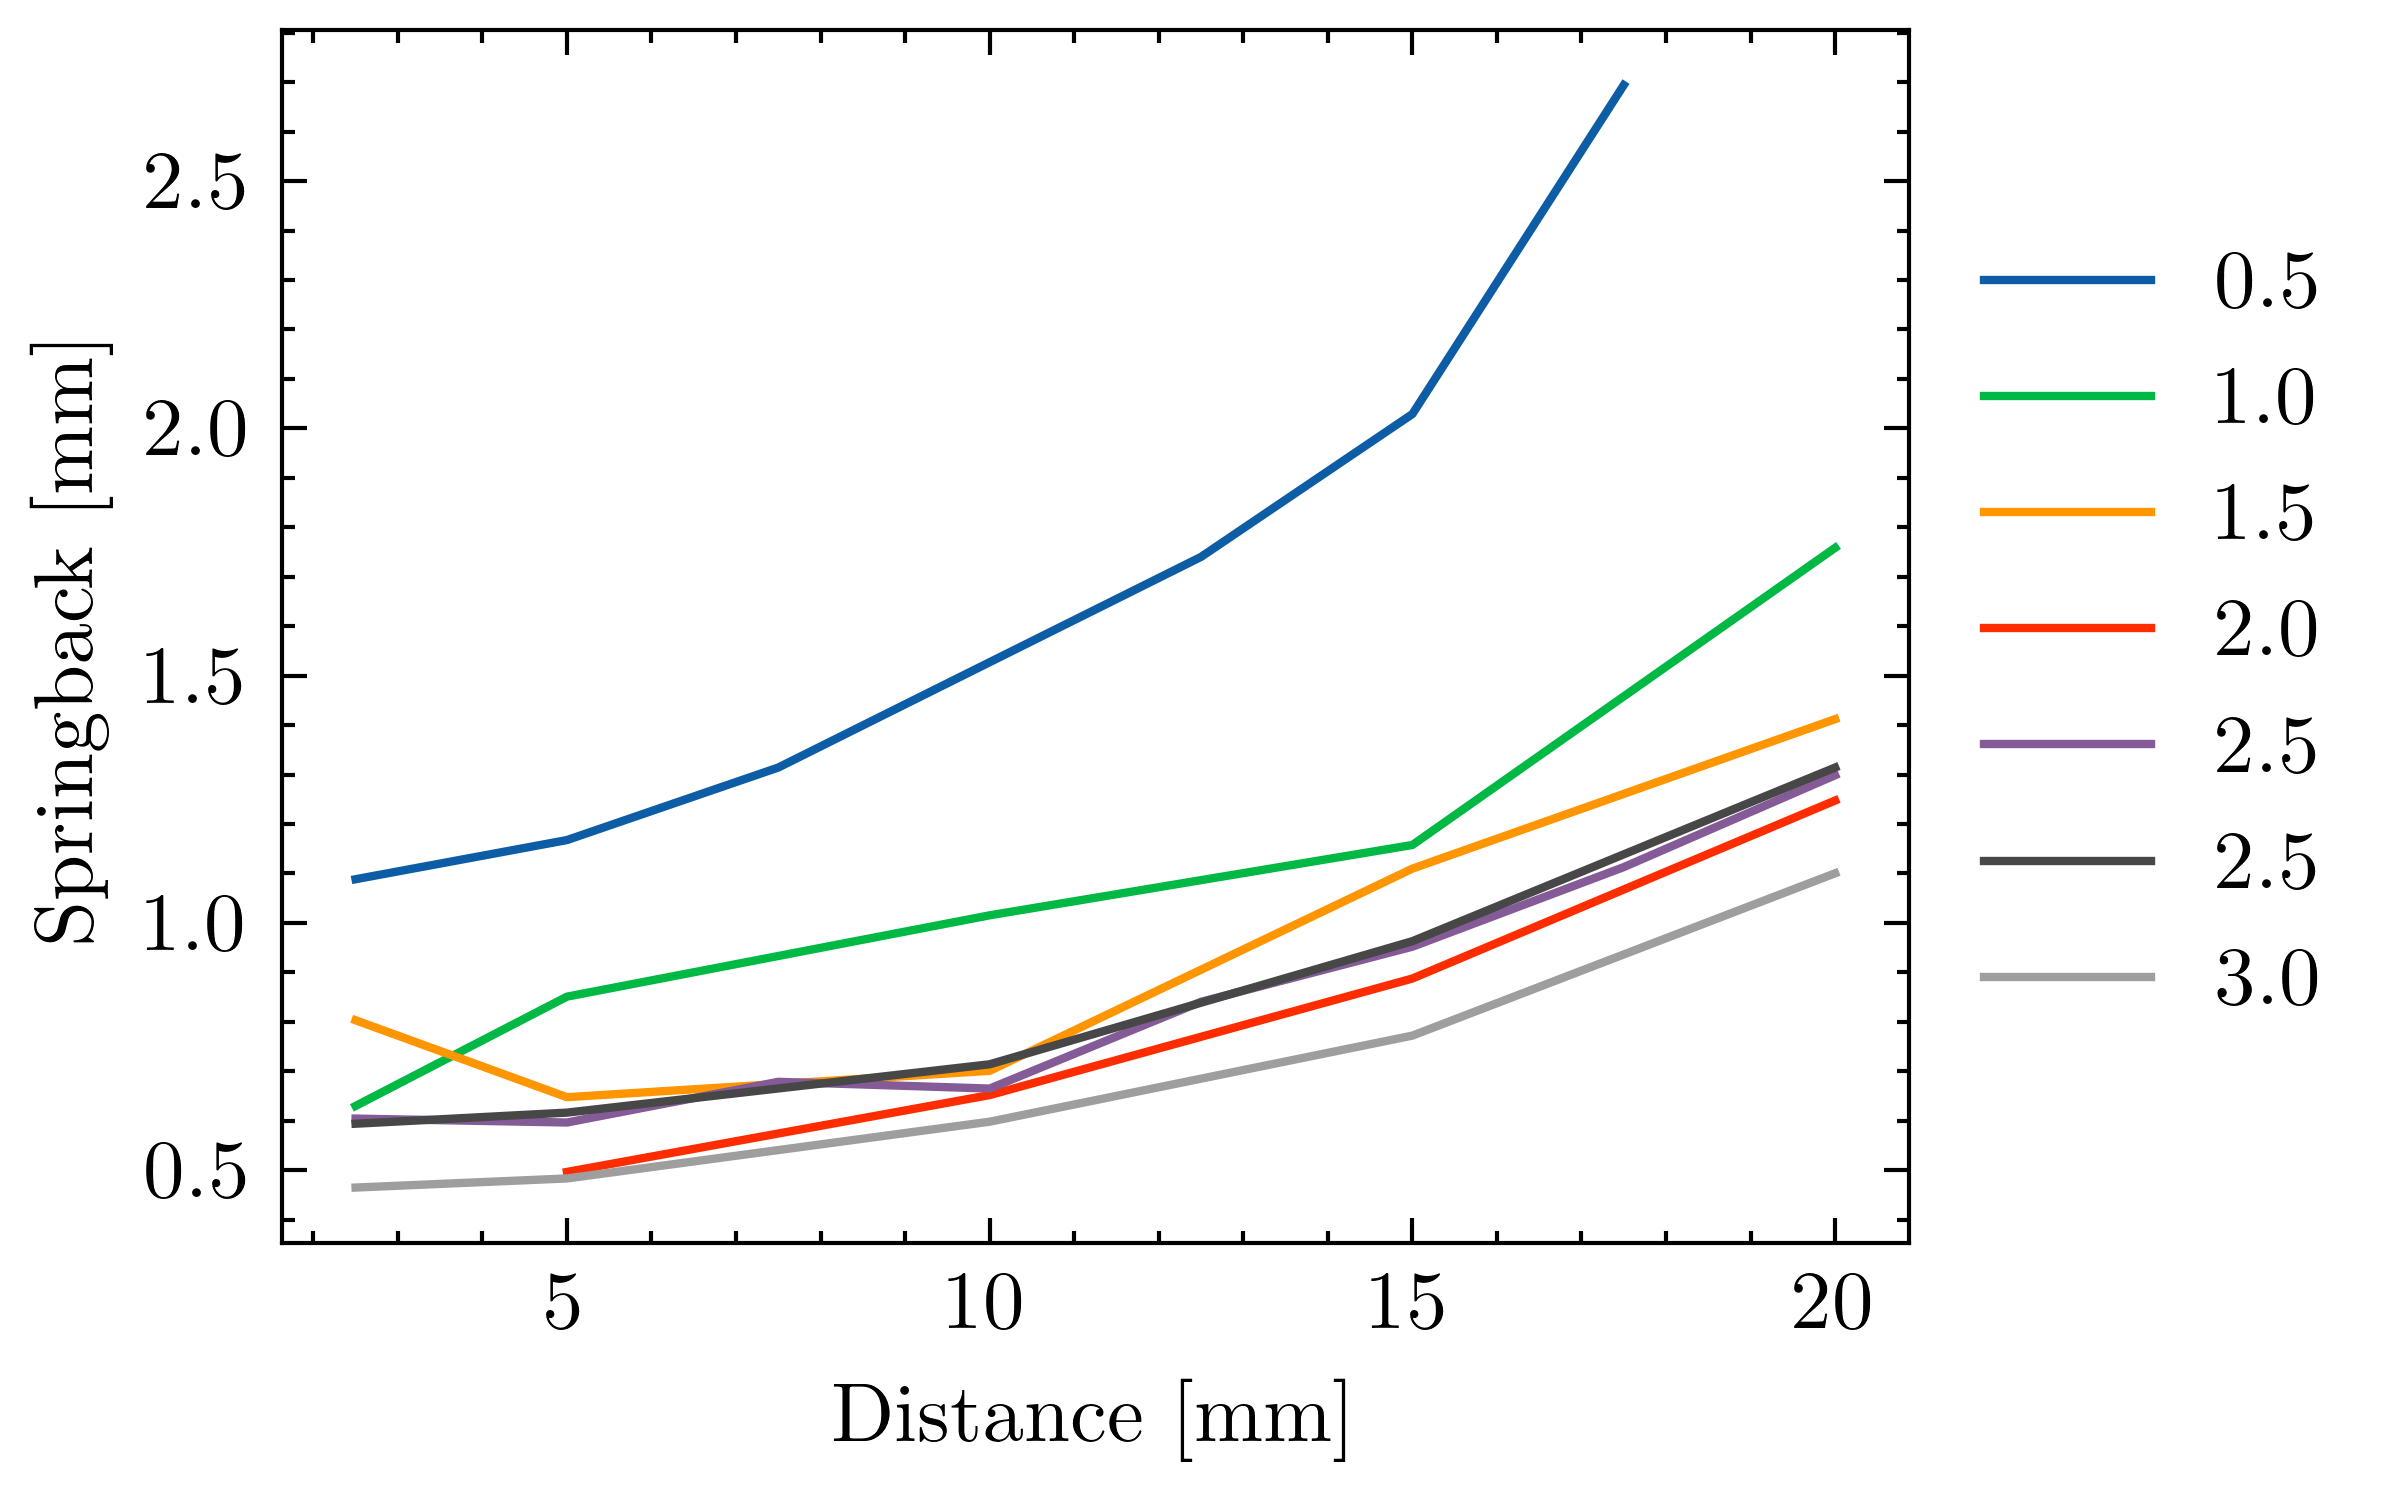
\includegraphics[width=0.9\textwidth]{all-springbacks-consolidated}
        \caption{Springbacks for $V30$}
        \label{fig:v30_springbacks}
    \end{tcolorbox}
\end{figure}

\subsubsection{Data Quality}
The dataset was created in a controlled experimental environment, where
was given to ensure that the samples were measured with precision and accuracy.
This results in a dataset that contains a minimal number of outliers and a
high level of data quality, which is an essential requirement for reliable machine
learning models.

As depicted in Figure~\ref{fig:train_test_split}, the dataset covers all possible
combinations of the process parameters, $V$, $t$ and $y_p$.
The $y_p$ values in the dataset are uniformly distributed and always range between 2.5
and 20 mm.
The dataset was continuously expanded with new data points throughout the project to
increase its size and diversity.

During the data collection and expansion process, several outliers and incorrect
measurements were identified and removed from the dataset to ensure its high quality.
Although this dataset has been developed in a controlled environment, it may not
accurately represent real-world scenarios, where the data quality is often affected by
a range of factors such as measurement errors, noise, and bias.
This will be taken into account in later sections, where data quality issues will be
added in order to evaluate the robustness of the models.

\subsection{Data Preprocessing}\label{subsec:data-preprocessing}
The three independent features $y_p$, $V$ and $t$ as well as the dependent
feature $spring\_back$ were normalized using the \texttt{MinMaxScaler} or in some cases
the \texttt{StandardScaler} from the \texttt{scikit-learn}\cite{scikit-learn} library.
The\texttt{MinMaxScaler} scales the data between 0 and 1.
The scaler was fitted on the training data and then used to transform the test data.
The scaler was saved to be used for the prediction of the spring back of the real world
data.

Scaling is only done on the training data, because cross-validation is later used to
tune and evaluate the models.
Scaling the whole data set before the split would lead to data leakage because the
minimum and maximum values of the test data would be used to scale the training data.
How the data was split can be seen in Figure~\ref{fig:train_test_split}.

\subsection{Computational Setup}\label{subsec:computational-setup}
For training the machine learning models a ThinkPad X1 Carbon 2019 with an
Intel Core i7-10610U CPU @ 1.80GHz and 16 GB RAM was used.
The operating system used is Ubuntu 20.04.2 LTS. The code for the model is
written in Python 3.8.5 using the IDE PyCharm.
The libraries used are mentioned in Table~\ref{table:libraries}.

\captionsetup{width=1\textwidth}

\begin{table}[htb]
    \begin{tcolorbox}[arc=0pt,boxrule=0.5pt]
        \sisetup{group-minimum-digits = 4}
        \centering
        \begin{tabular}{ll}
            \toprule
            \thead{\textbf{Library}} & \thead{\textbf{Version}} &
            \toprule
            numpy~\cite{harris2020array} & 1.23.2 \\
            \hdashline
            pandas~\cite{mckinney-proc-scipy-2010} & 1.5.1 \\
            \hdashline
            matplotlib~\cite{Hunter:2007} & 3.6.2 \\
            \hdashline
            scienceplots~\cite{SciencePlots} & 2.0.1 \\
            \bottomrule
        \end{tabular}
        \caption{Libraries used for the machine learning models.}
        \label{table:libraries}
    \end{tcolorbox}
\end{table}

Upon examining the correlation matrix depicted in Figure~\ref{fig:correlation_matrix},
it is evident that the distance and spring back features exhibit a stronger correlation
than the other features.
This correlation is to be expected since punch penetration $y_p$ is the primary factor
that influences the amount of spring back.
It is noteworthy that the other features are not correlated with each other, indicating
the absence of multicollinearity, which is a desirable trait for machine learning models.

\begin{figure}[H]
    \begin{tcolorbox}[arc=0pt,boxrule=0.5pt]
        \centering
        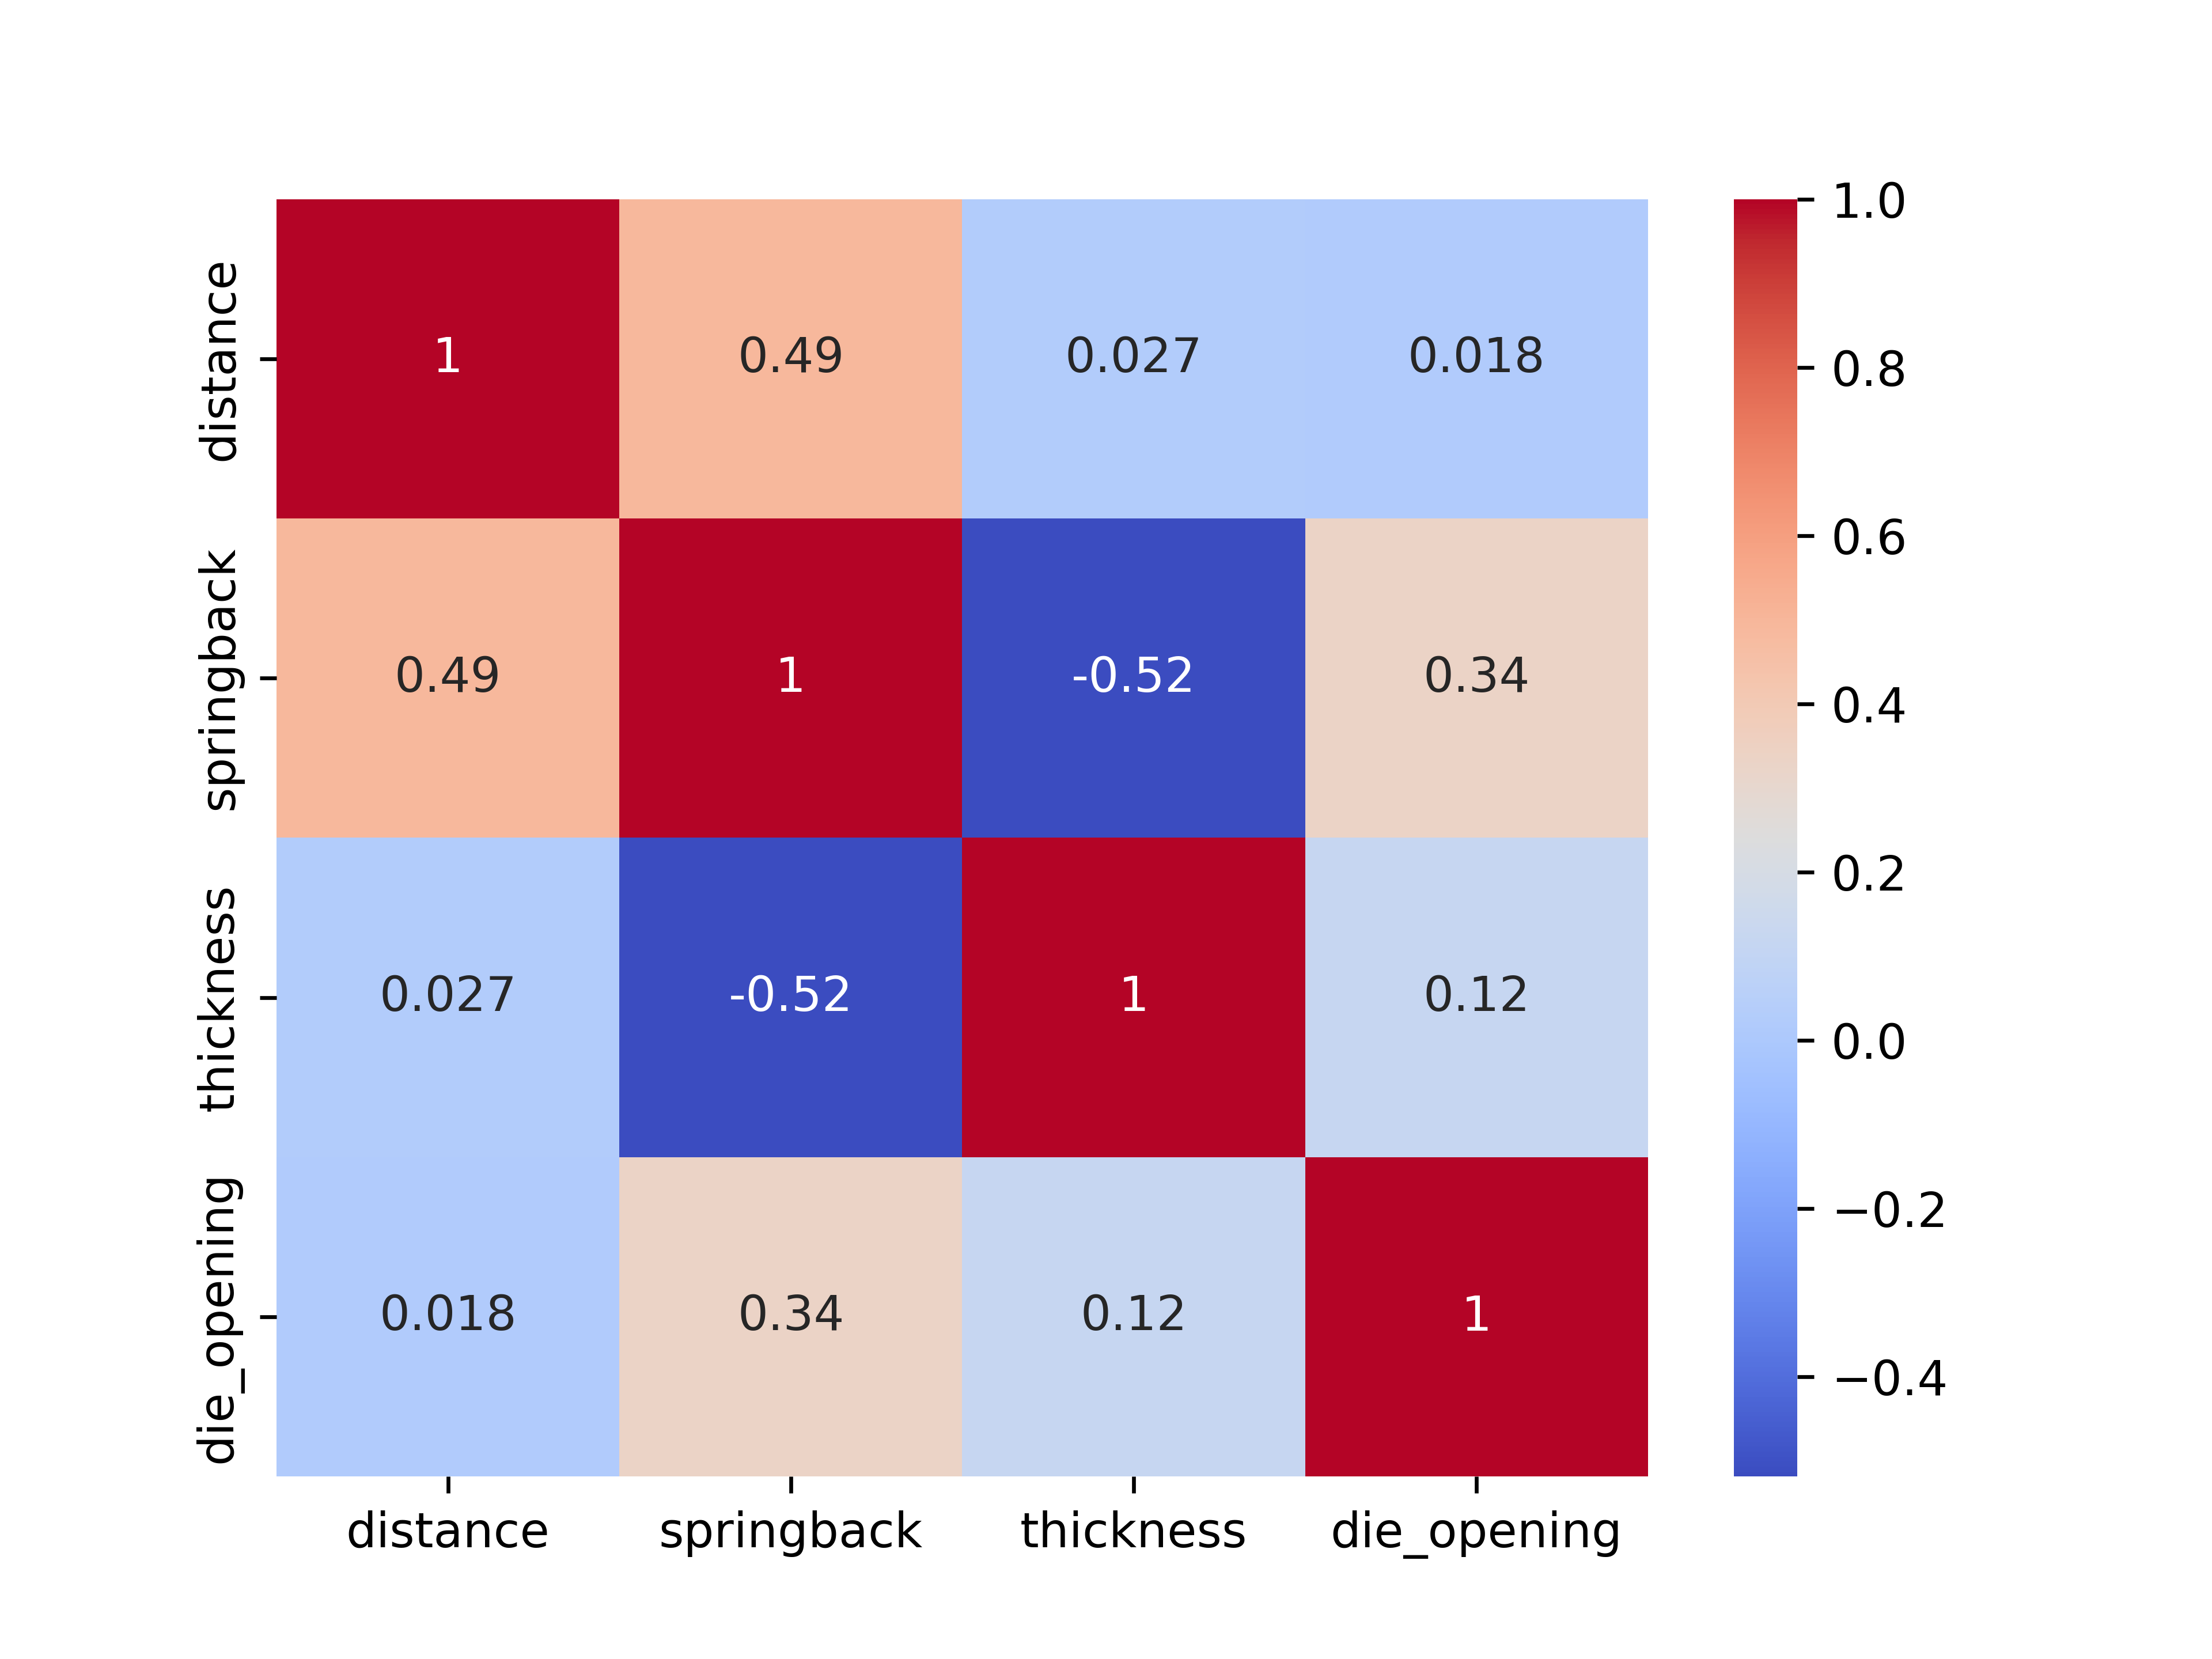
\includegraphics[width=0.7\textwidth]{correlation_matrix}
        \caption{Correlation matrix}
        \label{fig:correlation_matrix}
    \end{tcolorbox}
\end{figure}


\section{Model Selection}\label{sec:model-selection}
This thesis focuses on the utilization of supervised machine learning models to predict
spring back.
Therefore, a selection of the most common machine learning models where used, based on
the systematic literature review of~\cite{
    dridi2021supervised}.
In the paper, the author defines eight widely used supervised machine learning models: Logistic
Regression, Support Vector Machines, Decision Trees, Random Forests, AdaBoost, Naive Bayes, and K
-Nearest Neighbors~\cite[p. 8]{dridi2021supervised}.
However, Naive Bayes and K-Nearest Neighbors are not used in this thesis since they are typically
utilized for classification problems.
Furthermore, in order to compare the performance of the other models, a Linear Regression model
and a \ac{MLP} were also employed. The models can be classified into five categories: Logic-based
learning, instance-based learning, Deep learning, and Support Vector
Machines~\cite[p. 8]{dridi2021supervised}.

The author of the paper defines 8 widely used supervised machine learning models:
Logistic Regression, Support Vector Machines, Decision Trees, Random Forests, AdaBoost, Naive
Bayes and K-Nearest Neighbors~\cite[p. 8]{dridi2021supervised}.
Naive Bayes and K-Nearest Neighbors are not used in this thesis, because they are
generally used for classification problems.
Additionally a \ac{MLP} and Linear Regression model where are used to compare the performance of
the other models.
The models can be divided into five categories:
Logic-based learning, instance-based learning, static-based learning, Deep learning and
Support vector machines~\cite[p. 8]{dridi2021supervised}.

\subsection{Baseline Model}\label{subsec:regression-models}
In this thesis, a linear regression model is employed as the baseline model.
Linear regression is a straightforward and widely used method that is utilized for predicting
continuous values.
The model utilizes the feature inputs to generate a linear relationship that is both easy to
understand and interpret~\cite[p. 37]{molnar2020interpretable}.

To train the linear regression model, the sum of squared errors between the predicted values and
the actual values is minimized.
The mean squared error is determined by summing the squared differences between the predicted
values and the true values~\cite[p. 47--68]{muller_introductionmachinelearning_2016}.

The model is based on the assumption that the relationship between the independent
variables and the dependent variable is linear.
As previously mentioned in section~\ref{subsec:dataset-exploration}, the relationship between the
independent variables and the dependent variable is not linear.
Therefore, it is not anticipated that the linear regression model will produce accurate results.
However, the linear regression model is still used in order to evaluate the performance of the
other models.

Linear models can be used to understand the relationship between a target variable y
and one or more input features x.
The general formula for predicting in a linear model in regression is shown in
\ref{eq:linear-regression}~\cite[p. 45]{muller_introductionmachinelearning_2016}.
In this context, $x[0]$ to $x[p]$ represent the attributes (with p being the number of
attributes) of a specific data point.
The parameters $w$ and $b$, which are learned by the model, and the predicted output $\hat{y}$,
are also included~\cite[p. 45]{muller_introductionmachinelearning_2016}.

\begin{tcolorbox}[arc=0pt,boxrule=0.5pt]
    \begin{equation}
        \hat{y} = w[0] * x[0] + w[1] * x[1] + ... + w[p] * x[p] + b
        \label{eq:linear-regression}
    \end{equation}
\end{tcolorbox}

\ac{LR} models estimate the target value as linear combinations of the feature inputs.
The linearity of the relationship between the inputs and the target makes the
interpretation of the model straightforward~\cite[p. 37]{molnar2020interpretable}.

Linear regression has no hyper-parameters to tune and therefore no
hyperparameter tuning was performed.

%\subsection{Statistics Based Learning}\label{subsec:statistics-based-learning}
%
%The approach that relies on statistics and uses distributive statistics to make the
%problem more manageable.
%It predicts based on the distribution structure. Learning through statistics involves
%utilizing the Naïve Bayes Algorithm~\cite[p. 8]{dridi2021supervised}.
%
%\subsubsection{Naive Bayes}
%...

\subsection{Support Vector Regression (SVR)}\label{subsec:support-vector-regression-(svr)}
Support Vector Machines (\ac{SVM}) are a popular approach for solving classification
problems.
The algorithm seeks to identify a hyperplane in an N-dimensional space, where N
represents the number of features, to effectively separate and classify data
points.
The hyperplane divides the data into two classes, where the points on one side of the
hyperplane are classified as one class and the points on the other side are classified as
the other class~\cite[p. 42]{awad_efficientlearningmachines_2015}.

However, for regression problems such as predicting spring back, the \ac{SVM} algorithm
needs to be adapted to provide continuous values instead of a finite set of values.
To address this, the \ac{SVR} algorithm was developed, which draws inspiration from the
\ac{SVM} algorithm and leverages similar principles.
It fits a model to data by only considering residuals smaller in absolute value
than a designated constant known as $\epsilon$-sensitivity.
By doing so, \ac{SVR} can accurately model and predict continuous values, making it a
suitable approach for regression problems.

To enable the \ac{SVR} algorithm to generate continuous predictions, it creates a ``tube''
while the points outside the tube are penalized based on their distance from the
predicted function.
This approach is similar to how \ac{SVM}s penalize points in classification
problems~\cite[p. 369]{montesinoslopez_supportvectormachines_2022}.

% Kernel trick
To transform the data into a higher dimensional space a method called kernel trick is used.
Two methods are usually used for \ac{SVM}s, the polynomial kernel and the radial basis
function,also known as gaussian kernel~\cite[p. 97--98]{
    muller_introductionmachinelearning_2016}.
Similar to the \ac{SVM} algorithm, the \ac{SVR} algorithm finds a well-fitting hyperplane to a
kernel-induced feature space to achieve good generalization performance using the original
features.
This is detailed in~\cite[p. 369]{montesinoslopez_supportvectormachines_2022}.

The hyperparameters used for the algorithm in this work are listed in
table~\ref{tab:hyperparameters_svr}.

\begin{table}[H]
    \begin{tcolorbox}[arc=0pt,boxrule=0.5pt]
        \sisetup{group-minimum-digits = 4}
        \centering
        \label{tab:hyperparameters_svr}
        \begin{tabular}{ll}
            \toprule
            \thead{\textbf{Hyperparameter}} & \thead{\textbf{Value}} &
            \thead{\textbf{Description}}
            \\
            %  \unit{(Kcal\per\mole)\squared}}} & \thead{RMSD l.b.} &
            %  \thead{RMSD u.b.}  \\
            \toprule
            kernel & rbf
            \\
            \hdashline
            degree & 1
            \\
            \hdashline
            gamma & 0.1
            \\
            \hdashline
            C & 4000 \\
            \hdashline
            epsilon & 0.001 \\
            \bottomrule
        \end{tabular}
    \end{tcolorbox}
    \caption{Hyperparameters of the \ac{SVR} model}
\end{table}

\subsection{Logic-based learning}\label{subsec:logic-based-learning}

Logic-based algorithms solve problems by applying logical functions sequentially or
incrementally.
An example of such an algorithm is a decision tree, which is commonly used as a classification
and regression model~\cite[p. 10]{dridi2021supervised}.

\subsubsection{Decision Trees}
% -> Problem von decision tree
Decision Trees (\ac{DT}s) are a widely used type of model for both classification and
regression problems.
These models construct a hierarchy of rules to predict outcomes based on the data~\cite[p. 70]{
    muller_introductionmachinelearning_2016}~\cite[p. 253]{
    shaik_briefsurveyrandom_2019}.
In \ac{DT} models, the data is split into multiple segments based on specific feature
values.
This division creates various subsets of the dataset, with each sample
belonging to one subset.
The final subsets are called terminal or leaf nodes, while the intermediate subsets are
known as internal or split nodes.
To predict the outcome in a specific leaf node, the mean outcome of the training data
in that leaf node is used~\cite[p. 70--72]{muller_introductionmachinelearning_2016}.

Decision trees are models are useful when the relationship between features
and outcome is or when features interact with one another.
These models split the data multiple times based on certain cutoff values,
resulting in different subset of the dataset.
The final subsets, called leaf nodes are used to predict the outocme by
taking the average of the training data in that subset~\cite[p. 76]{
    molnar2020interpretable}.

\subsubsection{Random Forest}\label{subsubsec:random-forest-regression}
The main problem with \ac{DT} is their tendency to overfit and have poor
generalization performance, making them unsuitable for most use cases.
To address this, ensemble methods are typically used instead of a single DT~\cite[p. 78]{
    muller_introductionmachinelearning_2016}~\cite[p. 251]{liu_newmachinelearning_2012}.
% -> Warum random forst das problem löst
One popular ensemble learning algorithm is the \ac{RF}~\cite[]{
    breiman_randomforests_2001}, which combines multiple decision trees (weak learners
) to create a more accurate and stable prediction (strong learner)~\cite[p. 24]{
    awad_efficientlearningmachines_2015}.
Because the data is divided into smaller subsets, and a randomized tree predictor is
build for each subset this aproach is also called ``divide and conquer'' approach.
% -> Beschreibung Random forest / Random foret regression
The risk of overfitting is mitigated by using subset and feature randomization.
Each root node uses a unique subset of the data, and
each leaf is split using a random set of features.
This ensures that no single tree sees all of the data, allowing the model to focus on
general patterns rather than being
sensitive to noise~\cite[p. 251]{liu_newmachinelearning_2012}.

% -> Vorteile / Nachteile Random Forest
This mechanism is flexible enough to handle classifications and regression problems,
this is one of the reasons that random forests count to the most successful \ac{ML}
methods~\cite[p.
3-4]{biau_randomforestguided_2016}~\cite[p. 25]{breiman_randomforests_2001}.

%
% Advantages
%
Random forests are a type of machine learning algorithm that uses bagging and the
random selection of features to produce accurate results.
They are effective at handling noise and can work with both continuous and categorical
variables.
This combination of techniques helps improve the performance of the algorithm~\cite[p.
259]{liu_newmachinelearning_2012}.
Decision trees have a limitation in their ability to overfit, which is a
disadvantage.
his is mitigated by the use of subset and feature randomization.
Specifically, each base model uses a unique subset of the data, and each node in
the decision tree is split using a random set of features.
This ensures that no single tree sees all of the data, allowing the model to focus on
general patterns rather than being sensitive to noise~\cite[p. 259]{
    liu_newmachinelearning_2012}.

% Bagging technique helps the algorithms performance.
% Works well out of the box with no hyperparameter tuning.
% Fast, robust, and can show feature importances which can be quite useful.

% Disadvantages
%

% Boosted algos usuallaly outperform Random Forest.
% RF is not able to extrapolate based on the data. It can only predict within
% the range of the
% training data.
% Random forest regressor is unalbe to discover trens that would enable it in
% extrapolating
% values that fall outside
% of the training set.

%  Extrapolating is the process of estimating or predicting something beyond
%  the range of
%  available data. (chatgpt)

%
% Alogithm steps
%

% The following Random Forest Algorithm [9] gives the steps in constructing the
% decision trees.
% • Take N as the number of training data instances in the samples. Let M be the
% number of attributes in given input dataset.
% • Let m be the Number of parameter in the input that determines the next
% attribute
% to be chosen at each tree node; (where mislesserthan M).
% • The training samples are taken and a tree is constructed for each sample
% with
% replacement.
% • For tree node, arbitrarily select m attributes in that particular node.
% • The best split is computed based on the m input attributes of the sample
% dataset.
% • Each tree is grown without pruning.
% \cite[p. 254-255]{shaik_briefsurveyrandom_2019}

% A random forest does not require any cross verification and it is not
% over-fitting [8]. The
% Random forest uses Adaboost and Bootstrapping techniques to construct multiple
% classifiers. \cite[p. 254]{shaik_briefsurveyrandom_2019}


\subsubsection*{Hyperparameter Tuning}
Grid search cross validation was used to find the best hyperparameters for
the random forest model using Scikit-Learn's default \texttt{GridSearchCV} function.
All hyperparameters are summarized in Table~\ref{tab:hyperparameters_rf}.

The \textit{max\_features} was set to \textit{auto} and therefore the models
does use all available features.
As described in Figure~\ref{fig:rf_feature_importance} only limited features are
available and all of them are important for the dependent variable spring back
The default unpruned model did overfit the training data and therefore was not able to
generlaize well on new data (as decvitbed by \cite[p. 133-136]{
    muller_introductionmachinelearning_2016}).
There it was set to 10 using \texttt{GridSearchCV}.

\subsubsection{Gradient Boosting Regression Tree}
A gradient boosting regression is a type of ensemble learning algorithm in
which multiple decision trees are combines to produce a more accurate and stable
prediction.
Similar to the \ac{RF} gradient boosting combines multiple weak learners to create a
strong learner.
The difference to a \ac{RF} is, that the trees are trained in a serial manner and
each tree corrects the errors of the previous tree~\cite[p. 88--89]{
    muller_introductionmachinelearning_2016}.

Gradient boosted tree use strong pre-pruning and therefore produce shallow
trees with a depth of one to five.
This brings the advantage of a smaller model which uses less memory and also results in
a faster prediction.
Usually generating more trees improves the overall performance of the model~\cite[p.
88--89]{muller_introductionmachinelearning_2016}.
Also the algorithm performs well without scaling the dataset and can handle a mixture
of binary and continuous features~\cite[p. 88--89]{
    muller_introductionmachinelearning_2016}.
Like other tree-based models it does not perform well on high-dimensional data.

\ac{GBT} are more sen
"Gradient boosted trees are frequently the winning entries in machine
learning competitions, and are widely used in industry. They are
generally a bit more sensitive to parameter settings than random
forests, but can provide better accuracy if the parameters are set
correctly."~\cite[p. 88-89]{muller_introductionmachinelearning_2016}

"Apart from the pre-pruning and the number of trees in the ensemble,
another important parameter of gradient boosting is the learning rate,
which controls how strongly each tree tries to correct the mistakes of
the previous trees. A higher learning rate means each tree can make
stronger corrections, allowing for more complex models. Adding more trees to
the ensemble, which
can be accomplished
by increasing
n estimators, also increases the model complexity, as the model has
more chances to correct mistakes on the training set." \cite[p.
88-89]{muller_introductionmachinelearning_2016}

"The main parameters of gradient boosted tree models are the number
of trees, n estimators, and the learning rate, which controls the degree to
which each tree is
allowed to correct the
mistakes of the previous trees.
These two parameters are highly interconnected, as a lower
learning rate means that more trees are needed to build a model of
similar complexity. In contrast to random forests, where a higher
n estimators value is always better, increasing n estimators in gradient
boosting leads to a more complex model, which may lead to overfitting. A
common practice is to fit n estimators depending on the time and
memory budget, and then search over different learning rates." \cite[p.
88-89]{muller_introductionmachinelearning_2016}


\subsubsection*{Hyperparameter Tuning}
The \textit{kernel}, \textit{degree}, \textit{gamma} and \textit{epsilon}
where set using grid
search cross validation.
Gamma controls the width of the gaussian kernel, it determines when points
are close or far away.
The C parameter controls the importance of each point.

The features of the dataset have different order of magnitude, this is
already a problem for other
models, but big effects on the kernel \ac{SVM}.
To resolve this problem the data was scaled using the \textit{MinMaxScaler}
between 0 and 1.
The model trained on the scaled data performed better than the model trained
on the unscaled data.

\subsubsection{Extra Trees}\label{subsubsec:extra-trees}
When developing a tree within a random forest, only a portion of the features are
assessed for splitting at each node, which was previously explained in section~\ref{
    subsubsec:random-forest-regression}.
To further increase the randomness of the trees,
it is possible to utilize random thresholds for each feature rather than determining the
most optimal thresholds like traditional \ac{DT} do~\cite[p. 351]{geron2022hands}.

An ensemble of this kind highly arbitrary trees is known as an extra-trees (or extremely
randomized trees) ensemble.
This approach exchanges more bias for a lower variance.
Furthermore, the use of \ac{ET} classifiers makes the training process faster
compared to conventional random forests since one of the most time-intensive aspects of
tree development is determining the optimal threshold for each feature at
each node~\cite[p. 351]{geron2022hands}.

\subsection{Neural Networks}\label{subsec:neural-networks}
Another method for supervised learning involves the utilization of Neural Networks to
perform classification and regression tasks.
In this work the discussion will be limited on the use of relatively simple Multi-layer Perceptron.
MLPs can be seen as an extension of linear models that engage in several rounds of processing to
reach a conclusion~\cite[p. 104]{muller_introductionmachinelearning_2016}.

While this thesis does not delve into the use of Deep Learning for predicting spring
back, it does employ a simple multi-layer perceptron as a baseline model.
The results from this model can provide insights into the potential of neural networks for this
task and for guiding future research.

\subsubsection{Multi-layer Perceptron}
The multi-layer perceptron (MLP), which is the most widely used type of artificial
neural network, has to be found producing generalizable models in various fields~\cite[
    p.451]{taud2018multilayer}.

The MLP is a feedforward neural network that is organized into layers, with information
moving in one direction from the input layer trough the hidden layers to the output
layer~\cite{bishop1995neural}.
Each connection between neurons has a weight and perceptrons within the same layer
share the same activations function which is typically a sigmoid function in hidden
layers.

A backpropagation algorithm is typically used to train \ac{MLP} models, by
propagating errors backwards from the output layer to the input layer in order to adjust
the weights~\cite[p. 454]{taud2018multilayer}.

\section{Model Training}\label{sec:model-training}

\subsection{Training-Test Split}\label{subsec:training-test-split}
Figure~\ref{fig:train_test_split} displays the dataset partitioned into training and
testing sets for the models used in this study.
Specifically, the samples with a die
opening of 30 were reserved for testing, while the remaining data was used for training .
While a random train-test split can often yield better model performance, this
approach may not evaluate the model's ability to predict new data with a different die
opening.

The decision to use a die opening of 30 was based on its central location within the
selected dataset, allowing the models to predict this value accurately.
Furthermore,removing data from the middle of the parameter space during training is
expected to improve model performance and promote generalization to new data.

All models were trained on the same dataset. The hyper-parameters where set using Grid-Search Cross
-validation.
The full hyper-parameters for each model are listed in Table~\ref{sec:hyper-parameters}.

\begin{figure}[H]
    \begin{tcolorbox}[arc=0pt,boxrule=0.5pt]
        \centering
        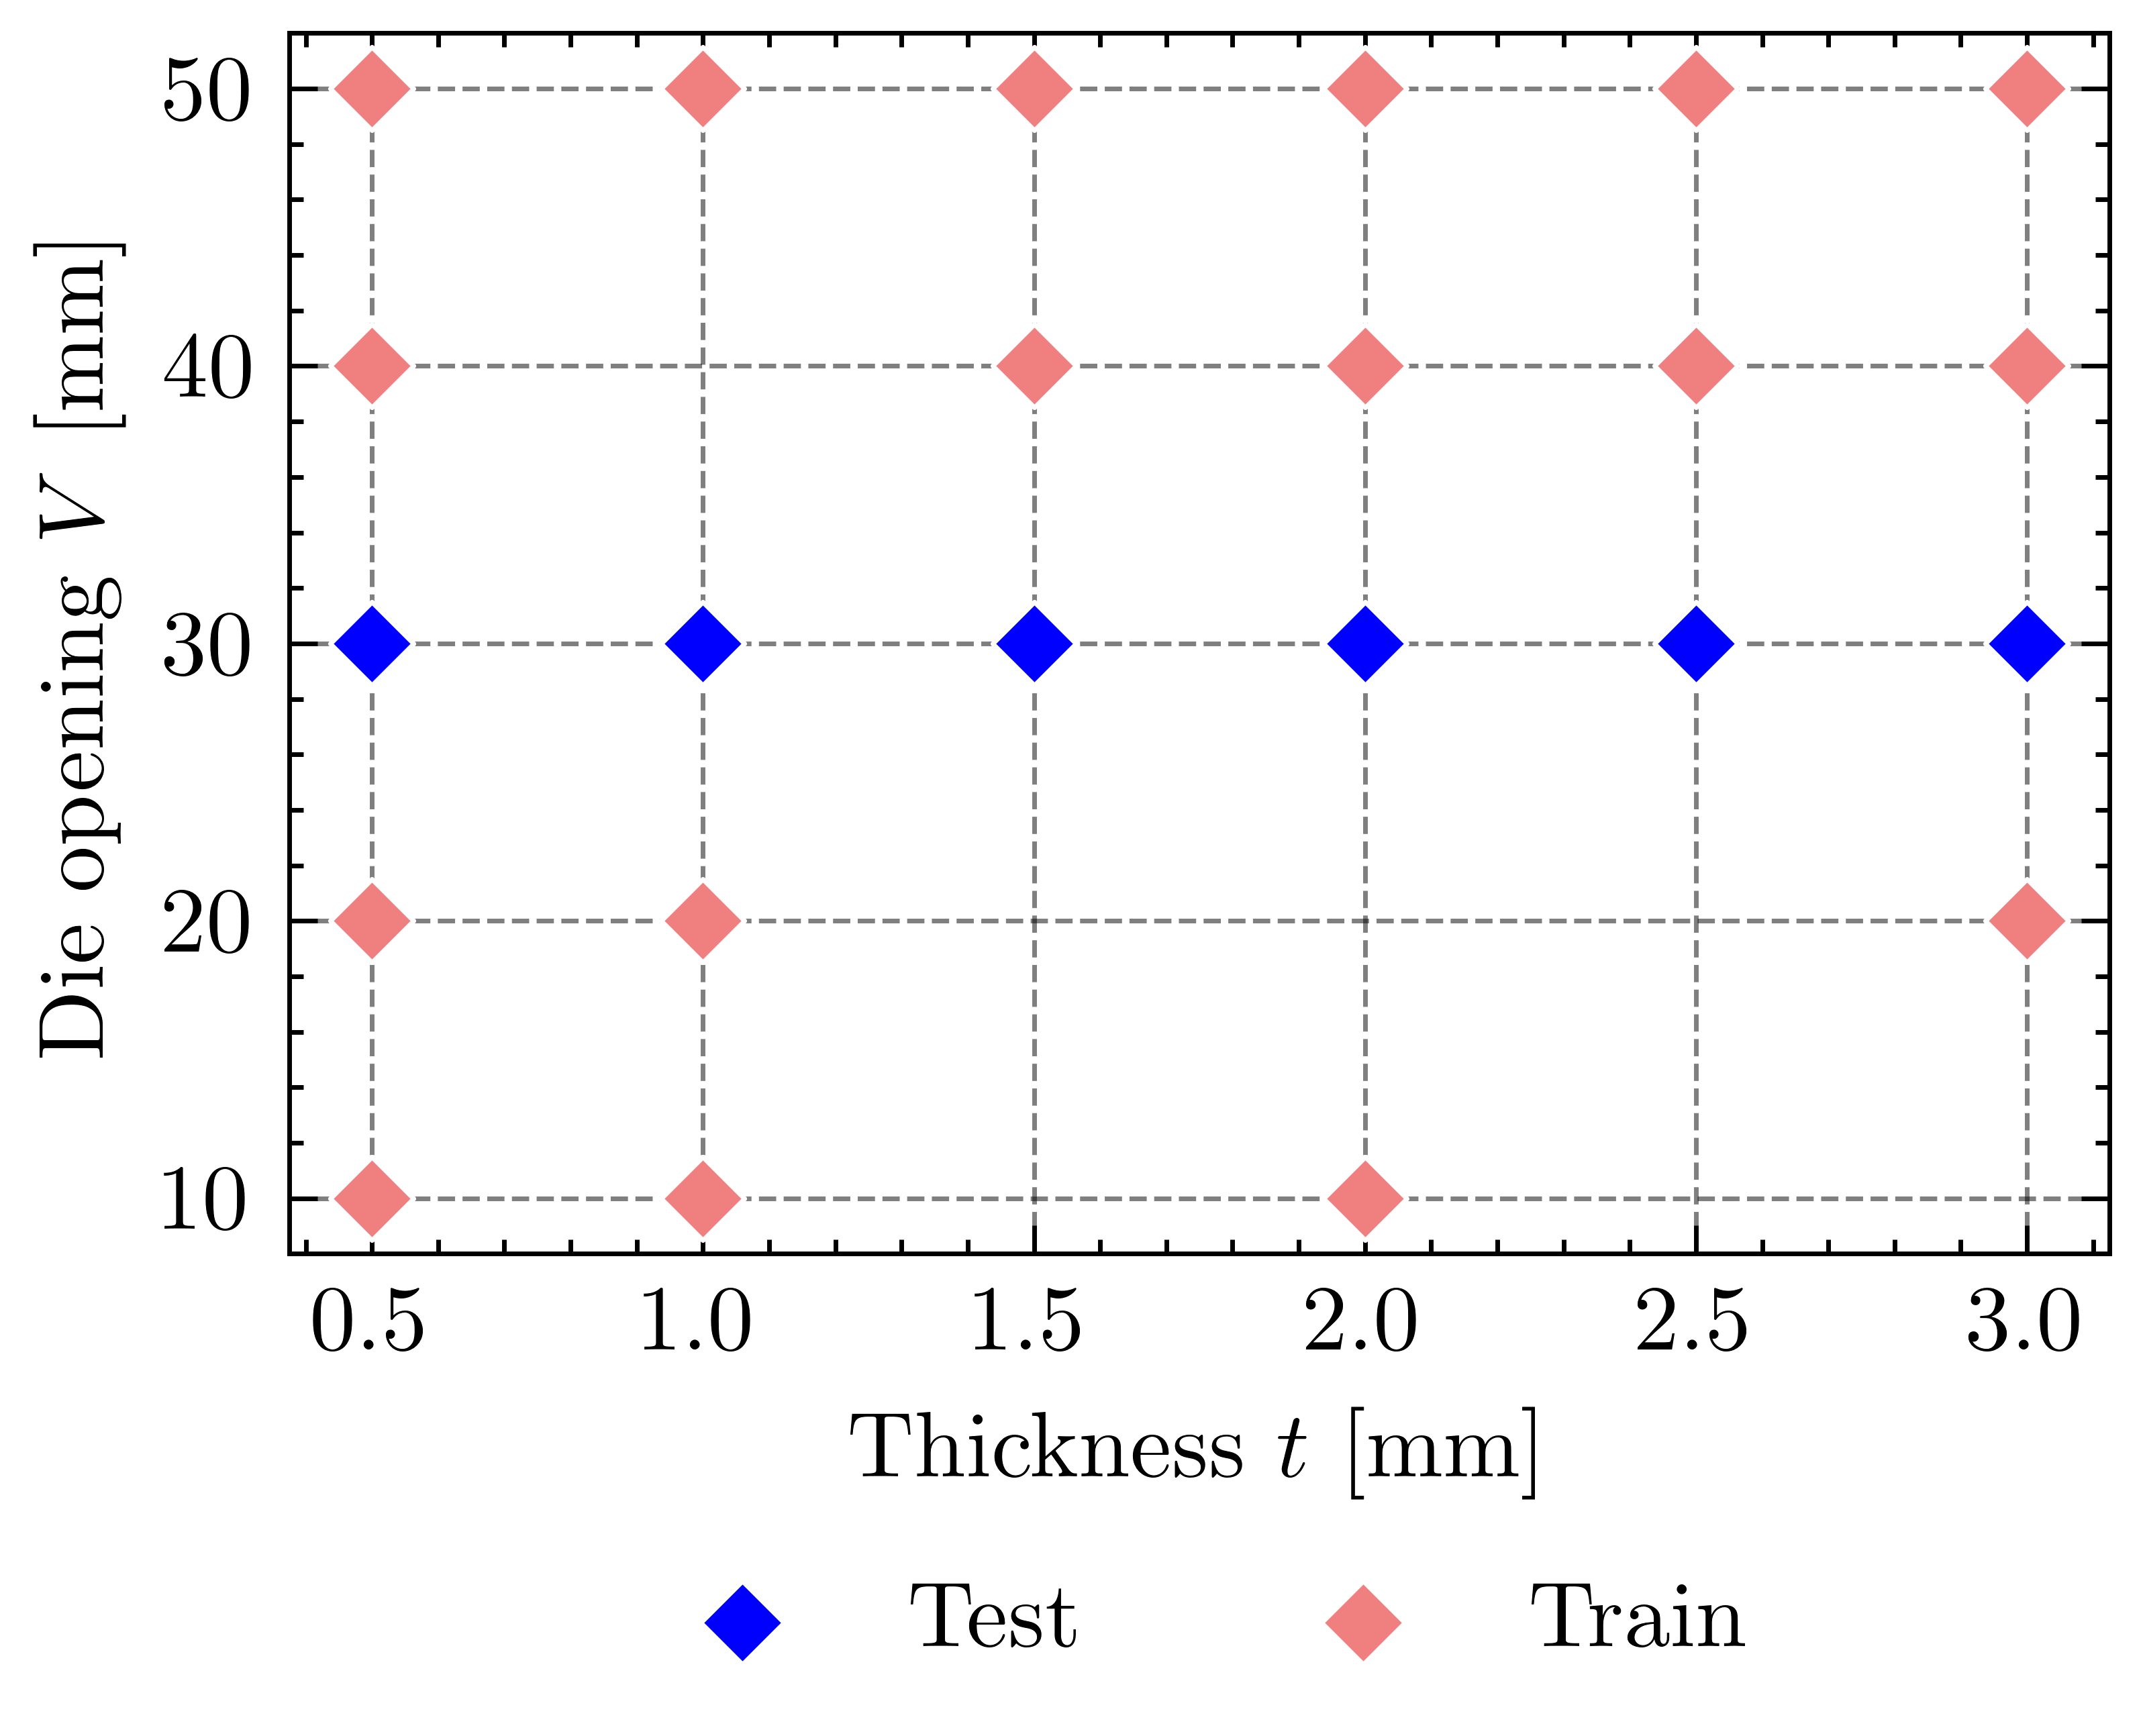
\includegraphics[width=0.8\textwidth]{test_train_split}
        \caption{The training and test dataset. (Data especially for V40 is
        still missing)}
        \label{fig:train_test_split}
    \end{tcolorbox}
\end{figure}

In addition to the data split shown in Figure~\ref{fig:train_test_split}, a random 80
/20 split was used to train and evaluate the models.
This split was employed to assess model performance and compare results.

Using two different methods for data splitting serves two distinct purposes.
The first method evaluates the models' ability to generalize on new data.
The second method assesses the models' performance on the dataset.
In real-world applications, it may be possible to train models on pre-existing data
that encompasses all necessary $V-t$-
combinations.

While the models are expected to perform better on the random data, less information
can be gained about their ability to generalize to new data because the random split
will most likely contain data from all $V-t$-combinations.


\section{Structure of The Code}\label{sec:structure-of-the-code}
The code is available on GitHub: \url{https://github.com/Philipp0205/Master-Thesis-Code}

The dataset can be found under the \texttt{data/dataset} folder.
All the used models are in the \texttt{learner} folder. Each learner class has a
\texttt{main} function which can be used to run the model.
Also the reports-array can be used to generate a specific report for the model.
The implementation of all reports can be found in the \texttt{reports} folder.

% \paragraph{Bend deduction:}
% Measuring the bend deduction is more complex. After a metal sheet is bent,
% it is hard to
% measure the flat pattern
% length because the material is malformed at the bent.
% As a result, the neutral axis is not in the center of the sheet and hard to
% measure, but it can
% be calculated using
% different approaches. %quelle und ausführlicher und grunlagen teil
% There are multiple ways to measure the bend deduction described earlier. 
% % K-Faktor Muss noch in theorie teil 
% In this setup, the method described in the DIN6395 was used. This method
% uses a k-factor which
% is an approximated
% value and therefore and therefore it can be inaccurate.
% (Equation~\ref{eq:kfactor}). % cite DIN
% norm

% \begin{equation}\label{eq:kfactor}
%     k=0.65+\frac{1}{2}\log{\frac{r}{s}}
% \end{equation}

% \begin{figure}[ht!] % supposedly places it here ...
% 	\centering
% 	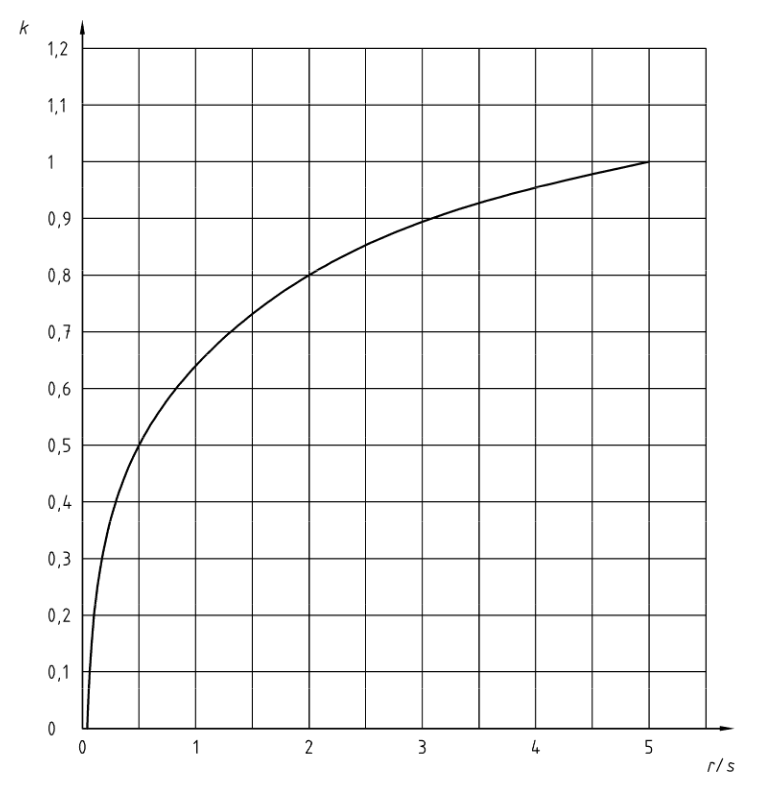
\includegraphics[width=0.5\linewidth]{k-factor}
% 	\caption[Graphical representation of the correction factor]{Graphical
% representation of the
% correction factor.}
% 	\label{fig:test1}
% \end{figure}

% The DIN 6935 used the formula for the stretched length, $length=a+b+v$
% where \textit{a} and
% \textit{b} are the side
% lengths of the sheet and \textit{v} is a correction value for the deduction
% . \cite{din6935}
% The stretched length is measured different depending on the bending angle.

% \paragraph{Opening angle $\beta 0^\circ$ to $90^\circ$} 
% For opening angles between $0^\circ$and $90^\circ$ the side lengths
% \textit{a} and \textit{b}
% are dimensioned from
% the tangent of the bend to the edge.
% To calculate the compensation value \textit{v} (Equation~\ref{eq:v1}) is used
% \cite{din6935}.

% \begin{equation}\label{eq:v1}
%         v=\pi*(\frac{180^\circ-}{180^\circ})*(r+\frac{s}{2}*k)-2(r+s)
% \end{equation}

% \begin{figure}[H]
% 	\centering
% 	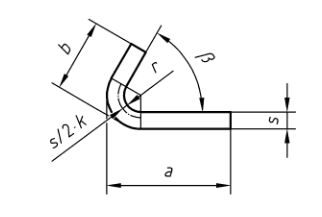
\includegraphics[width=0.5\linewidth]{bending-angle-90}
% 	\caption[Opening angles $\beta 0^\circ$ to $90^\circ$]{Opening angles
% $\beta 0^\circ$ to
% $90^\circ$ \cite{din6935}}
% 	\label{fig:v1-image}
% \end{figure}

% \paragraph{Bending angle $\beta90^\circ$ to $165^\circ$}
% (Equation~\ref{eq:v1})
% For opening angles between $90^\circ$ and $165^\circ$ the side lengths
% \textit{a} and
% \textit{b} are dimensioned
% from the apex to the edge.
% To calculate the compensation value \textit{v} (Equation~\ref{eq:v1}) is
% used.
% \cite{din6935}

% \begin{equation}\label{eq:v2}
%     v=\pi*(\frac{180^\circ-}{180^\circ})*(r+\frac{s}{2}*k)-2(r+s)
% +\tan{\frac{180^\circ-\beta}{2}}
% \end{equation}

% \begin{figure}[!ht]
% 	\centering
% 	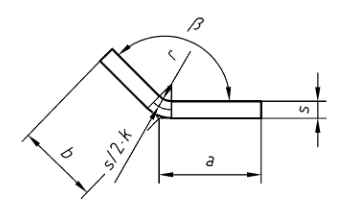
\includegraphics[width=0.5\linewidth]{bending-angle-165}
% 	\caption[Opening angles $\beta90^\circ$ to $165^\circ$]{Opening angles
% $\beta90^\circ$ to
% $165^\circ$
% \cite{din6935}}
% 	\label{fig:v2-image}
% \end{figure}

% For opening angles between $165^\circ$ and $180^\circ$ the compensation
% value \textit{v} is 0.
% The values for v
% would be negligibly small. \cite{din6935} The side lengths \textit{a} and
% \textit{b} where
% measured using the
% software \textit{ImageJ}.

% Edge cracking is not measured for now because the steel used has no
% high-strength and with
% machine in usage it was
% not possible to create edge cracking.

% \begin{figure}[!ht]
% 	\centering
% 	\includegraphics[width=0.5\linewidth]{example-image}
% 	\caption[Screenshot ImageJ]{Screenshot ImageJ}
% \end{figure}
% 	\label{fig:imagej-screenshot}